%*****************************************
\chapter{Analysis of incentive policies for phosphorus recovery}\label{ch:Policies}
%*****************************************
\begin{refsection}[referencesCh5]
\section*{Abstract}
Livestock operations have been highly intensified over the last decades, resulting in the advent of large concentrated animal feeding operations (CAFOs). Intensification decreases production costs but also leads to substantial environmental impacts. Specifically, nutrient runoff from livestock waste results in eutrophication, harmful algal blooms, and hypoxia. The implementation of nutrient recovery systems in CAFOs can abate nutrient releases and negative ecosystem responses, although they might negatively affect the economic performance of CAFOs. We design and analyze potential incentive policies for the deployment of phosphorus recovery technologies at CAFOs considering the geospatial vulnerability to nutrient pollution. The case study demonstration consists of 2,217 CAFOs in the U.S. Great Lakes area. The results reveal that phosphorus recovery is more economically viable in the largest CAFOs due to economies of scale, although they also represent the largest eutrophication threats. For small and medium-scale CAFOs, phosphorus credits progressively improve the profitability of nutrient management systems. The integration of biogas production does not improve the economic performance of phosphorus recovery systems at most of CAFOs, as they lack enough size to be cost-effective. Phosphorus recovery proves to be economically beneficial by comparing the net costs of nutrient management systems with the negative economic impact derived from phosphorus releases. The incentives necessary for avoiding up to $20.7 \cdot 10^3$ ton/year phosphorus releases and achieve economic neutrality in the Great Lakes area are estimated at \$223 million/year. Additionally, the fair distribution of limited incentives is studied using a Nash allocation scheme, determining the break-even point for allocating monetary resources.

\bigskip
\textbf{Keywords:} Organic waste; Incentive policy; Environmental policy; Livestock industry; Phosphorus recovery; Circular economy
\newpage

\section*{Resumen}
Las explotaciones ganaderas se han intensificado mucho en las últimas décadas, lo que ha dado lugar a la aparición de grandes explotaciones concentradas de alimentación animal (CAFO). La intensificación disminuye los costes de producción, pero también provoca importantes impactos ambientales. En concreto, la escorrentía de nutrientes procedente de los residuos ganaderos provoca eutrofización, floraciones de algas nocivas e hipoxia. La implantación de sistemas de recuperación de nutrientes en las CAFO puede reducir las emisiones de nutrientes y las respuestas negativas del ecosistema, aunque podría afectar negativamente a los resultados económicos de las CAFO. Diseñamos y analizamos posibles políticas de incentivos para la implantación de tecnologías de recuperación de fósforo en las CAFO teniendo en cuenta la vulnerabilidad geoespacial a la contaminación por nutrientes. El caso de demostración consiste en 2.217 CAFO en la zona de los Grandes Lagos de Estados Unidos. Los resultados revelan que la recuperación de fósforo es más viable económicamente en las CAFO más grandes debido a las economías de escala, aunque también representan las mayores amenazas de eutrofización. Para las CAFO de pequeña y mediana escala, los créditos de fósforo mejoran progresivamente la rentabilidad de los sistemas de gestión de nutrientes. La integración de la producción de biogás no mejora el rendimiento económico de los sistemas de recuperación de fósforo en la mayoría de las CAFO, ya que carecen del tamaño suficiente para ser rentables. La recuperación de fósforo demuestra ser económicamente beneficiosa al comparar los costes netos de los sistemas de gestión de nutrientes con el impacto económico negativo derivado de las emisiones de fósforo. Los incentivos necesarios para evitar hasta $20.7 \cdot 10^3$ toneladas/año de vertidos de fósforo y lograr la neutralidad económica en la zona de los Grandes Lagos se estiman en 223 millones de dólares/año. Además, se estudia la distribución justa de los limitados incentivos mediante un esquema de asignación de Nash, determinando el punto de equilibrio para la asignación de los recursos monetarios.

\bigskip
\textbf{Palabras clave:} Residuos orgánicos; Políticas de incentivos; Políticas ambientales; Industria ganadera; Recuperación de fósforo; Economía circular
\newpage


\section{Introduction}
In the context of continuous human population growth, an efficient and sustainable food production system becomes a key factor to guarantee social welfare. Currently, intensive livestock farming produces most of the meat and dairy products worldwide, and the demand is expected to double by 2050 compared to 2007 \citep{livestock_projection}. To meet this increasing demand, the development of intensive farming practices has resulted in the concentrated animal feeding operations (CAFOs) \citep{animal_unit_definition}, which allows larger and cheaper productivity than traditional systems. However, concerns in terms of food safety, animal health, and environmental impacts are associated with intensive livestock farming. Focusing on environmental impacts, livestock industry needs large amounts of water, represents 14.5\% of the anthropogenic-based GHG emissions \citep{eisler_agriculture:_2014}, and is a source of nutrient releases which lead to high concentrations of phosphorus in soil and waterbodies \citep{Sampat2017}. Focusing on nutrient pollution, phosphorus releases by improper organic waste management from livestock facilities contribute largely to the eutrophication of fresh and marine waters, promoting harmful algal blooms (HABs) which can release toxins and cause the hypoxia of waterbodies as a result of algae biomass decomposition. 
Therefore, the development of sustainable agricultural intensification techniques is not only a desirable but also a necessary measure to reduce the environmental impact of livestock industry while meeting the current and future food demand. In this regard, the implementation of integrated systems for manure management can recover valuable components contained in livestock waste, including phosphorus and biogas-based products, and the environmental footprint of CAFOs is decreased.

From a technical perspective, the adoption of nutrient management systems in CAFOs is feasible, but their practical implementation has to overcome several other logistical  and economic barriers.
Therefore, developing effective incentive policies to support the economic sustainability of livestock facilities plays a critical role in the successful adoption of phosphorus recovery technologies.
This is especially relevant because, despite the additional capital and operating costs these processes entail for the CAFOs, long-term remediation expense up to 74.5 USD per kg of released phosphorus \citep{Sampat2020} can be avoided by recovering phosphorus before it reaches soil and waterbodies. Remediation costs are believed to not affect the owners of livestock facilities directly; however, environmental remediation costs are usually covered by public budgets funded by taxpayers, and may lead to the eventual application of specific taxes on livestock products for their environmental footprint.

Nowadays, most of efforts to abate nutrient releases into the environment and mitigate the eutrophication of waterbodies are focused on the limitation of fertilizer application in croplands.
In the United States, CAFOs are regulated under the Clean Water Act as point source waste discharges. This regulation sets the need of permits for discharging pollutants to water, called National Pollutant Discharge Elimination System (NPDES) permits, including the release of nitrogen of phosphorus. This permit must include the necessary provisions for avoiding the harmful effects of the discharges on water and human health \citep{NPDE_basics}. The development and implementation of a Nutrient Management Plan (NMP) is a required element to obtain a NPDES permit. This document must identify the management practices to be implemented at the CAFO to protect natural resources from nutrient pollution. Land spreading of manure can also be regulated by the NPDES permits, establishing soil nutrient concentration limits and the yearly schedule for manure application. However, no specific waste treatment methods or processes are defined under federal regulation  \citep{NPDESforCAFO}. Regarding the use of the recovered nutrients, the products obtained from nutrient recovery processes could be classified as waste by the Clean Water Act, preventing the application of these materials on croplands \citep{NACWA503}. However, the US Environmental Protection Agency (US EPA) determined that, although these products could not be directly applied to land under the current regulation, they can be sold as a commodity to be outside of the scope of Clean Water Act restrictions. Moreover, US EPA acknowledges that highly refined and primarily inorganic products (such as struvite) could be outside the scope of these restrictions \citep{CNP503}. However, further regulation is needed to define the products obtained from nutrient recovery processes and to clearly define the conditions for their use as fertilizers on croplands.

In the European Union (EU), the application of fertilizer and manure for
%nitrogen supplementation is currently regulated by the Nitrates Directive (91/676/EEC) \citep{GRIZZETTI2021102281}. Regarding the limitations for phosphorus application, these 
phosphorus supplementation
is defined at national level. Several European countries, including Belgium, Denmark, Germany, the Netherlands, Sweden, and Norway, among others, have implemented application standards based on the different crops and materials used as fertilizers. Generally, phosphorus application limits are more restrictive in northwestern Europe \citep{amery2014agricultural}. 
%It can be observed that nutrient application is limited either in the form of synthetic fertilizers or manure application. However, at present there is a lack of regulation regarding livestock waste treatment \citep{Piot_Lepetit2012}.
Although nutrient application in croplands is limited either in the form of synthetic fertilizers or manure, there is a lack of regulation regarding livestock waste treatment \citep{Piot_Lepetit2012}.
However, similarly to the US, new efforts for the adoption of bio-fertilizers obtained from organic waste are currently underway in the development of the ``Integrated Nutrient Management Plan" (INMAP), which is part of the EU Farm-to-Fork strategy and part of the Circular Economy Action Plan. INMAP should propose actions to promote the recovery and recycling of nutrients, as well as to accelerate the development of markets for the recovered nutrients \citep{ESSP2021, CircularEconomyActionPlan}. In this regard, a new regulation for fertilizer products has been released in 2019 (EU 2019/1009), which moves struvite and other biofertilizers from the category of waste to fertilizers, and establishes a regulatory framework for their use and trade.

In sum, the regulation of the products obtained from nutrient recovery systems is not totally developed yet, although important efforts are being performed in order to set a comprehensive regulatory framework for the recycling of phosphorus. However, no regulation regarding the implementation of nutrient recovery processes has been developed either in the EU and the US.
%Different incentive schemes can be considered to promote the adoption of sustainable nutrient management systems, including phosphorus releases allowances in the form of P credits and renewable electricity certificates (REC) for energy recovery.

In this work, a systematic analysis of different incentive schemes for implementing phosphorus recovery systems at CAFOS is performed through a computational framework for the techno-economic analysis of nutrient and energy recovery technologies for livestock facilities. Suitable nutrient and energy recovery technologies are determined for each studied CAFO among the state-of-the-art processes for organic waste management. The effect of different incentive policies on the economic performance of nutrient management technologies is studied considering the environmental vulnerability to nutrient pollution in the Great Lakes area. Additionally, the combination of incentives for the recovery of both phosphorus and electricity has been considered to identify potential synergies between the different technologies involved in the processing of livestock waste. The results obtained allow for the identification of the optimal incentive policies for the implementation of sustainable nutrient management systems at CAFOs as a function of their size, type of animals, and the environmental vulnerability of the area where each studied CAFO is located. In addition, we study the allocation of limited monetary resources  using a Nash scheme; this determines the break-even point for the allocation of monetary resources based on the availability of incentives.

%\section{Review of current policies}
%Attending to the regulatory aspect, nowadays most of the efforts for abating of nutrient releases into the environment and mitigating the eutrophication of waterbodies are focused in the limitation of fertilizer application in croplands. The application of fertilizer and manure for nitrogen supplementation en the European Union (EU) is currently regulated by the Nitrates Directive (91/676/EEC) \citep{GRIZZETTI2021102281}. Regarding the limitations for phosphorus application, these are defined at national level. Several European countries have implemented application standards based on the different crops and materials used as fertilizers. Generally, phosphorus application limits are more restrictive in northwestern Europe \citep{amery2014agricultural}. It can be observed that nutrient application is limited either in the form of synthetic fertilizers or manure application. However, at present there is a lack of regulation regarding livestock waste treatment \citep{Piot_Lepetit2012}. New efforts for the adoption of bio-fertilizers obtained from organic waste are being currently performed in the development of the "Integrated Nutrient Management Plan" (INMAP), which is part of the part of the EU Farm-to-Fork strategy and part of the Circular Economy Action Plan. INMAP should propose actions to promote the recovery and recycling of nutrients, as well as the development of markets for recovered nutrients \citep{ESSP2021, CircularEconomyActionPlan}. In this regard, a new regulation for fertilizer products has been released in 2019 (EU 2019/1009), moving struvite and other biofertilizers from the category of waste to fertilizers, establishing a regulatory framework for their use and trade.
%
%In the United States, CAFOs are regulated under the Clean Water Act as point source waste discharge. This regulation sets the need of permits for discharging pollutants to water, called National Pollutant Discharge Elimination System (NPDES) permits, including the release of nitrogen of phosphorus. This permit must include the necessary provisions for avoiding the harmful effects of the discharges on water and human health \citep{NPDE_basics}. The development and implementation of a Nutrient Management Plan (NMP) is a required element to get a NPDES permit. This document must identify the management practices to be implemented at the CAFO to protect natural resources from nutrient pollution. Land spreading of manure can also be regulated by the NPDES permits, establishing soil nutrient concentration limits and the yearly schedule for manure application. However, no specific methods or processes are defined under federal regulation \citep{NPDESforCAFO}. Regarding the use of the recovered nutrients, products obtained from nutrient recovery processes could be classified as waste ny the Clean Water Act, preventing the application of these materials on croplands \citep{NACWA503}. However, U.S. Environmental Protection Agency (US EPA) determined that, although these products could not be directly applied to land under the current regulation, they can be sold as a commodity to be outside of the Clean Water Act restrictions coverage. Moreover, US EPA acknowledges that highly refined and primarily inorganic products (such as struvite) could be outside of the scope of these restrictions \citep{CNP503}. However, further regulation is needed for defining the products obtained from nutrient recovery processes and to clearly state the conditions for their use as fertilizers on croplands.

\section{Incentive policy assessment framework}

A two-stage framework is proposed for the evaluation of incentive policies, as shown in Figure \ref{fig:tool_diagram}. 
In the first stage, the selection of
%In the first stage, the size and geographical location of the studied CAFOs are analyzed, selecting
the most suitable P recovery process for each CAFO assessed is performed based on the size and geographical location of CAFOs. Process selection has been performed using a multi-criteria decision analysis (MCDA) model developed in a previous work \citep{Tool}. This system integrates geographic data for determining the environmental vulnerability to nutrient pollution, and the technical and economic information of the nutrient recovery systems to determine the most suitable P recovery technology for each studied CAFO. Firstly, the type and number of animals in each studied CAFO, as well as their geographical location, are entered into the model (box \textit{a}). 
%The assessment of the regional environmental vulnerability to nutrient pollution is carried out in a
A geographic information system (GIS) model (box \textit{b}) evaluates the regional environmental vulnerability to nutrient pollution. This model is
% through three indicators, i.e, , 
described in Section \ref{section:EnvVulNutPol}.
Additionally, a techno-economic assessment of the different phosphorus recovery technologies, and biogas production in those cases where this process is considered, is performed based on the characteristics of the CAFO in parallel (box \textit{c}). The evaluated processes are shown in Section \ref{section:TEAPRec}.
%The information returned by these models is normalized and aggregated in a MCDA model to select the most suitable nutrient management technology for each evaluated livestock facility (box \textit{d}). 
To select the most suitable P recovery system at each CAFO, the information from the techno-economic analysis and the geographical assessment of the vulnerability to nutrient pollution is combined in an MCDA model (box \textit{d}), which is described in Section \ref{section:MCDAPRec}. In this model, both phosphorus recovery cost and efficiency of the systems under evaluation are balanced as a function of the environmental vulnerability to
eutrophication of each region. As a result, the minimization of operating costs is prioritized in regions with low vulnerability to nutrient pollution, whereas the selection of phosphorus recovery technologies with larger recovery efficiencies is prioritized in regions affected by nutrient pollution, even if they incur in larger recovery costs.
%consist of a multi-criteria decision analysis (MCDA) model integrating a geographic information system (GIS)-based model for determining the environmental vulnerability to nutrient pollution, and the techno-economic analysis (TEA) of phosphorus recovery technologies. We note that these technologies can be implemented either standalone, or integrated with anaerobic digestion (AD) for biogas production.

In a second stage, this model has been extended to design and analyze
%the effect of different 
incentive policies for
%phosphorus recovery on the nutrient recovery processes selected
the deployment of the P recovery technologies selected in the first stage. The effect of incentives on the economic performance of the P recovery systems is evaluated
%
%The P recovery selection stage is composed of different models that are fed with data regarding the type and number of animals in the studied CAFO, as well as its geographical location (box \textit{a}). The techno-economic assessment of the different phosphorus recovery technologies, and biogas production in those cases where this process is considered, is performed based on the characteristics of the CAFO (box \textit{b}). Additionally, the assessment of the regional environmental vulnerability to nutrient pollution is carried out in a parallel stage (box \textit{c}). The information returned by these models is normalized and aggregated in a multi-criteria decision analysis (MCDA) model to select the most suitable nutrient management technology for the evaluated livestock facility (box \textit{d}). 
%The stage analyzing the impact of incentives on the economic performance of the nutrient management systems is comprised 
by an economic model that estimates their profit,
%systems implemented
capital expenses (CAPEX), operating expenditures (OPEX), and phosphorus recovery cost
%of the processes for P recovery selected for each studied CAFO.
at each CAFO under study.
Additionally, a cost-benefit analysis comparing the recovery cost and the economic losses due to nutrient pollution is performed (box \textit{e}).
%Section 1 of the Supplementary Information.

\begin{figure}[h!]
	\centering
	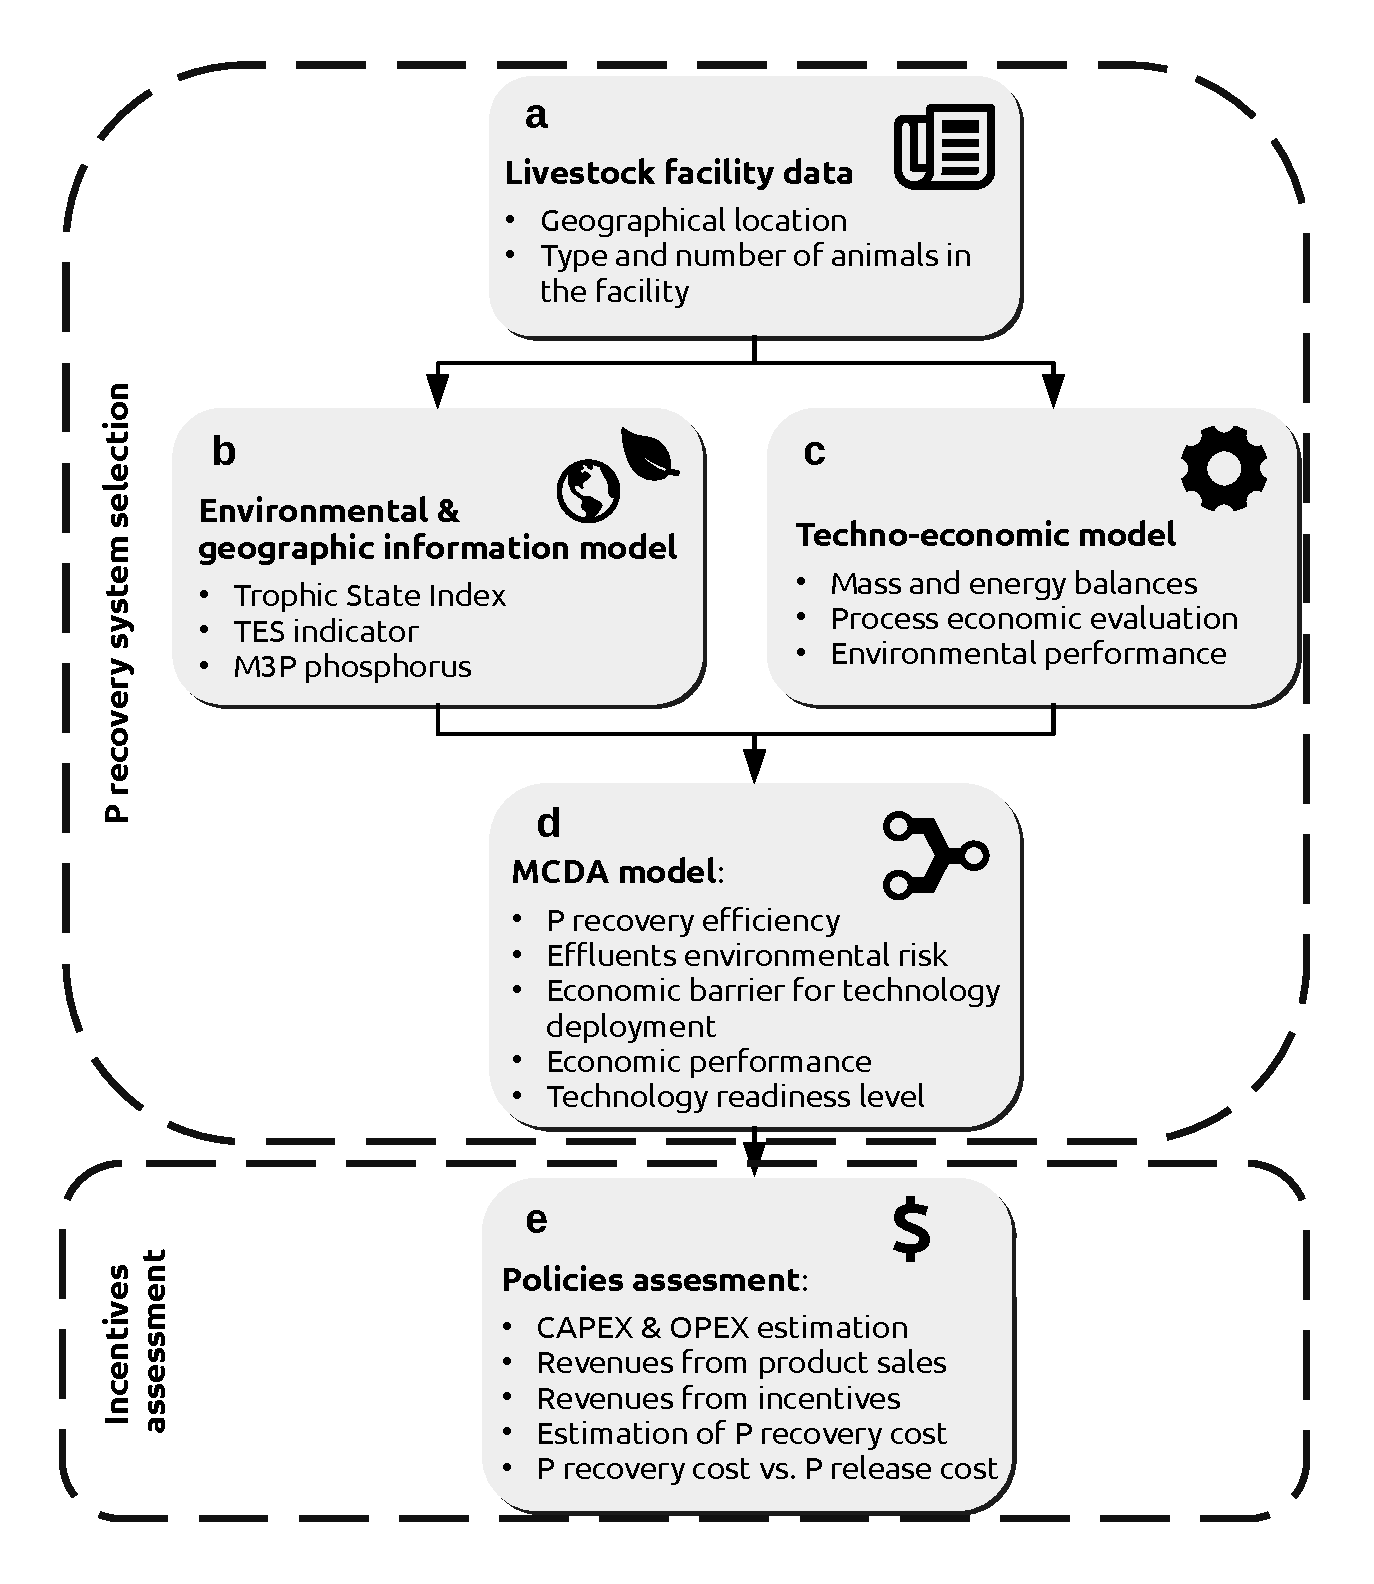
\includegraphics[width=0.7\linewidth, trim={1cm 1cm 1cm 1cm},clip]{gfx/Chapter5/tool_diagram_v4colorClean.pdf} 
	\caption{Flowchart of the models for selection, sizing, and evaluation of nutrient recovery systems at livestock facilities.}
	\label{fig:tool_diagram}
\end{figure}

\subsection{Assessment of nutrient management systems}
Figure \ref{fig:techs_diagramsPaperIncentives} illustrates the processes considered for livestock waste management. These processes comprise all manure treatment stages from waste collection to phosphorus recovery, including the optional biogas production stages. For the sake of brevity, a brief description of the processes is provided in this section. A detailed description of the framework employed for the assessment of nutrient management systems can be found in \citet{Tool}.

\begin{figure}[h!]
	\centering
	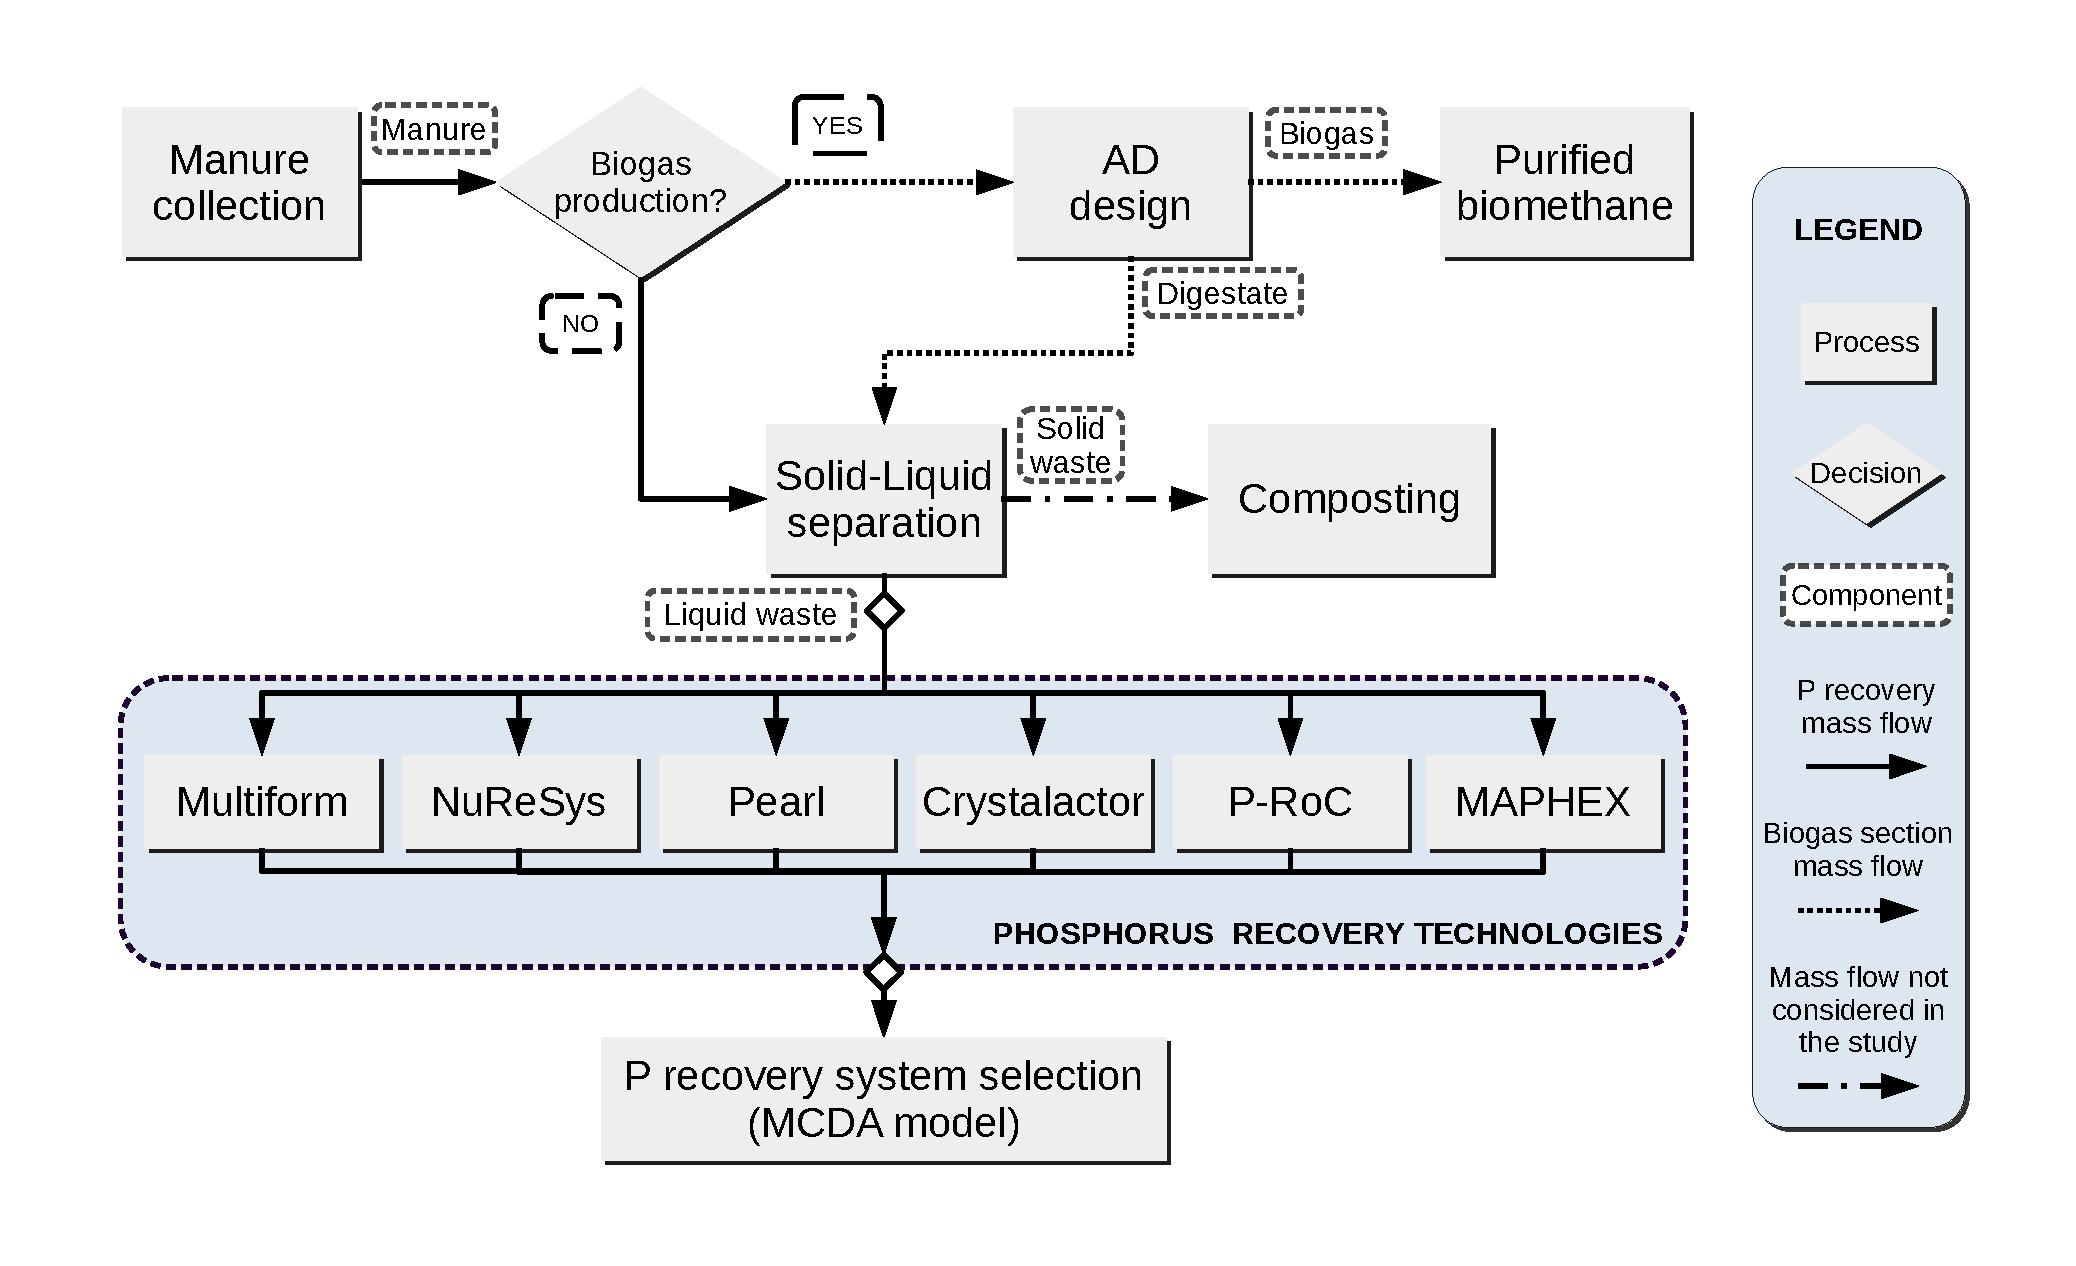
\includegraphics[width=0.85\linewidth, trim={1.5cm 1.5cm 1.5cm 1.5cm},clip]{gfx/Chapter5/Process_FlowsheetClean.pdf} 
	\caption{Flowchart of the processes evaluated for livestock waste management.}
	\label{fig:techs_diagramsPaperIncentives}
\end{figure}

\subsubsection{Environmental vulnerability to nutrient pollution}\label{section:EnvVulNutPol}
A
%geographic information system (GIS)
GIS model is developed to estimate the environmental vulnerability to nutrient pollution of the area where each studied CAFO is located. We have considered three dimensions of phosphorus pollution to determine the eutrophication risk in each studied watershed, (i) the average Trophic State Index (TSI) of the waterbodies in the studied area \citep{carlson_trophic_1977}, (ii) the legacy of phosphorus in soils measured by the Mehlich 3 phosphorus (M3P) concentration \citep{Espinoza2006}, and (iii) the balance between phosphorus releases and uptakes derived from human activities using the the techno-ecological synergy (TES) metric \citep{TESmetric}. These parameters have been evaluated at a sub-basin spatial scale, which corresponds to the HUC8 level defined in the Hydrologic Unit Code (HUC) system \citep{HUC8}. The information retrieved by this environmental GIS-based model is used to set the priority of environmental and economic criteria, as described in the next section. A detailed description of the GIS model used to estimate the vulnerability to nutrient pollution can be found in \citet{Tool}.
%the section 2.2 of the Supplementary Material.

\subsubsection{Techno-economic analysis of phosphorus recovery systems}\label{section:TEAPRec}

Six state-of-the-art technologies are assessed for phosphorus recovery at CAFOs. These technologies can be classified into three categories, i.e. struvite-based phosphorus recovery (Multiform, Crystalactor, Ostara Pearl, and NuReSys), calcium precipitates-based phosphorus recovery (P-RoC), and physical separation systems (MAPHEX). Table \ref{table:techs_description} summarizes the main parameters of the P recovery technologies assessed. In addition, nutrient management technologies can be implemented either as standalone systems, or integrated with biogas production and upgrading processes, being both scenarios considered in this work. In those scenarios in which the integrated nutrient-energy recovery processes are considered, biogas is produced through AD of cattle waste. In a second stage, biogas impurities (mainly $\text{H}_2 \text{S}$, $\text{NH}_3$, and moisture) are eliminated, and carbon dioxide is removed using a pressure swing adsorption (PSA) unit. A detailed description for the modeling of AD and biogas purification processes can be found in \citet{Leon}, while the modelling of the PSA system is shown in \citet{MartinHernandez}.

The different processes, including solid-liquid separation, biogas production, and phosphorus recovery systems, are modeled based on first principles, which include mass and energy balances, thermodynamics, and product yield calculations. Additionally, data from manufacturers have been considered when available, particularly for the estimation of 
%capital expenses (CAPEX) and operating expenditures (OPEX).
the equipment and operating costs. The techno-economic parameters computed in this stage for each process include the amount of phosphorus recovered, the eutrophication potential of the process effluents, the net present value (NPV), and the technology readiness level (TRL).
A review and modeling details of the technologies considered can be found in \citet{Tool}.
%Section 2.3 of the Supplementary Information.

\begin{table}[]
	\centering
	\caption{Description of phosphorus recovery technologies considered in this work. $x_{Ca^{2+}:PO_{4}^{3-}}$ refers to the $\text{Ca}^{2+}/\text{PO}_{4}^{3-} \ \text{molar ratio}$.}
	\label{table:techs_description}
	\resizebox{\columnwidth}{!}{
		\begin{tabular}{@{}ccccc@{}}
			\toprule
			P recovery process & \begin{tabular}[c]{@{}c@{}}Technology\\ readiness level\end{tabular} & Technology type                                                                     & \begin{tabular}[c]{@{}c@{}}Phosphorus recovery\\ efficiency (\%)\end{tabular} & Reference \\ \midrule
			Multiform          & 9                          & Struvite                                                                                                & $\frac{0.798 \cdot 100}{1+\left(x_{Ca^{2+}:PO_{4}^{3-}} \cdot 0.576\right)^{2.113}}$                                   &  \citep{Pearl2Kcost2}          \\
			Crystalactor       & 9                          & Struvite                                                                                                & $\frac{0.798 \cdot 100}{1+\left(x_{Ca^{2+}:PO_{4}^{3-}} \cdot 0.576\right)^{2.113}}$                                   & \citep{egle_phosphorus_2016}          \\
			NuReSys            & 9                          & Struvite                                                                                                & $\frac{0.798 \cdot 100}{1+\left(x_{Ca^{2+}:PO_{4}^{3-}} \cdot 0.576\right)^{2.113}}$                                   &  \citep{Pearl2Kcost2}         \\
			Pearl              & 9                          & Struvite                                                                                                & $\frac{0.798 \cdot 100}{1+\left(x_{Ca^{2+}:PO_{4}^{3-}} \cdot 0.576\right)^{2.113}}$                                   & \citep{Pearl2Kcost2}           \\
			P-RoC              & 6                          & Calcium precipitates                                                                                    & 60                                   &  \citep{ehbrecht_p-recovery_2011}         \\
			MAPHEX             & 7                          & \begin{tabular}[c]{@{}c@{}}Modular system based on\\ phases separation\end{tabular}                          & 90                                   &     \citep{church_novel_2016}      \\ \bottomrule
	\end{tabular}}
\end{table}

%\subsubsection{Biogas production and upgrading}
%In addition, nutrient management technologies can be implemented either as standalone systems, or integrated with biogas production and upgrading processes, being both scenarios considered in this work. In those scenarios in which the integrated nutrient-energy recovery processes are considered, biogas is produced through AD of cattle waste. In a second stage, biogas impurities (mainly $\text{H}_2 \text{S}$, $\text{NH}_3$, and moisture) are eliminated, and carbon dioxide is removed using a pressure swing adsorption (PSA) unit. A detailed description for the modeling of AD and biogas purification processes can be found in \citet{Leon}, while the modelling of the PSA system is shown in \citet{MartinHernandez}.
%A comprehensive description for the PSA system and its modeling is shown in \citet{MartinHernandez}.


\subsubsection{Multi-criteria decision analysis model for the assessment of nutrient management systems} \label{section:MCDAPRec}
The model developed for the evaluation and selection of on-site processes for the treatment of livestock waste is based on a MCDA model.
%multi-criteria decision analysis (MCDA) framework. 
This model combines the information from the techno-economic assessment and the local environmental vulnerability to nutrient pollution. Five parameters which can be classified in three dimensions are evaluated to select the most suitable P recovery process for each CAFOs; i.e.,  (i) environmental dimension assessing the performance of the different technologies to mitigate phosphorus releases from CAFOs, which measured through the fraction of phosphorus recovered by each technology (criterion 1), and the eutrophication potential of its effluents (criterion 2), (ii) the economic performance of the P recovery systems, including the economic barrier for the implementation of P recovery processes measured in terms of capital cost (criterion 3), and the net present value (NPV) of each process (criterion 4), and (iii) the technical maturity of each system, measured through the technology readiness level (TRL) index (criterion 5).

We developed a flexible criteria aggregation method able that balances the operating cost of the systems and the P recovery efficiency as a function of the environmental vulnerability to eutrophication of each region through criteria prioritization. In order to promote the implementation of proven P recovery processes, the TRL index is set as the criteria with highest preference in all cases. Regarding the environmental and economic aspects, environmental criteria are prioritized in the MCDA module if high values for TSI or M3P are reported for the area of study, which result in severe environmental risk of phosphorus pollution. As a consequence, the selection of phosphorus recovery technologies with larger recovery efficiencies is prioritized even if they incur in larger capital or operating expenses. On the other hand, economic criteria are prioritized for technology selection either of the following situations happens, (a) if the trophic state of waterbodies is oligotrophic or mesotrophic and therefore there is no immediate eutrophication risk, but phosphorus emissions and uptakes are unbalanced, or (b) no environmental risk is reported.

For each studied CAFO, the normalized criteria are combined following the preference method described above. As a result, we obtain a composite index for each P recovery technology that collects the information of the criteria considered. 
Based on the value of this composite index, these processes can be compared and ranked, selecting the most suitable system for each studied CAFO. Detailed descriptions for the construction of composite indexes can be found in  \citet{HandbookCompositeIndicators}. 

In order to achieve a robust decision for the selection of the most adequate phosphorus recovery process, a sensitivity analysis considering different methods for the normalization and aggregation of economic and environmental information is performed \citep{MarcoCinelli2020}. A comprehensive description of the MCDA model for the selection of phosphorus recovery systems according to the economic and environmental parameters of each CAFO is collected in \citet{Tool}.
%Section 2.4 of the Supplementary Information.

\subsection{Types of incentives considered}
The implementation of nutrient recovery incentives in the form of phosphorous credits (P credits) has been studied in this work. In addition, in those scenarios where biogas production is integrated, renewable electricity certificates (REC) are also considered.

P credits can provide a mechanism to promote the recovery of phosphorus that is similar to the carbon credit scheme used in the context of carbon emissions, leading to the development of a credits market around phosphorus releases. The acquisition of P credits can bring allowances for phosphorus releases. Conversely, an entity can obtain income by recovering phosphorus releases, which is the P credits definition considered in this work. Previous efforts to determine the impact of implementing phosphorus recovery incentives for livestock waste management supply chain networks have been addressed by \citet{sampat_economic_2018}. An optimal value of 22 USD per kg of phosphorus recovered is proposed to ensure the profitability of nutrient management systems implemented at CAFOs. Additionally, since the deployment of phosphorus recovery systems results in marketable nutrient-rich products in the form of struvite, incomes from the sale of these products are included in the calculation of revenues.

REC incentives for energy recovery provide a fixed remuneration for the electricity produced, which can result in a higher transaction price of electricity to cover the extra production costs and guarantee long-term price stability. Many different REC values have been proposed by governmental organizations worlwide based on geographical factors and power production capacity \citep{Deremince}. Therefore, similar to the electricity market price, a value of 60 USD/MWh, has been considered as baseline price.

\subsection{Scenarios description}
A total of 36 scenarios combining incentives in the form of phosphorus credits (0, 1, 3, 5, 11, and 22 USD/${\text{kg}_\text{P recovered}}$) and for the production of electricity (considering final electricity prices of 30, 60, 75, 90, and 120 USD/MWh) are evaluated for the implementation of nutrient management systems at 2,217 CAFOs in the Great Lakes area. The base value assumed for P credits is 22 USD per kg of phosphorus recovered, based on the work of \citet{sampat_economic_2018}. Although this reference value is comparatively large with respect to the price of phosphorus in commercial fertilizer, 1.23 USD/kg P \citep{fertilizers_price}, we note that it is significantly lower than the economic losses due to the environmental and social impact of nutrient pollution, estimated to be 74.5 USD per kg of P released \citep{Sampat2020}. Regarding RECs, an average electricity market price of 60 USD/MWh has been selected as the base-scenario. An electricity price below this value, 30 USD/MWh, and three values above the electricity market price, 75, 90, and 120 USD/MWh have been considered. These high REC values are studied due to the need of large incentives for biogas facilities to be economically viable reported by \citet{sampat_economic_2018}.

We note that there are two special cases among the scenarios assessed. For those scenarios where P credits are 0, the only income of phosphorus recovery is from the sales of marketable nutrient-rich products in the form of struvite, in addition to the incomes from electricity generated if the corresponding technologies are selected. For those scenarios with an electricity price of 0 USD/MWh, no biogas production and upgrading process is implemented, considering only incomes associated with P credits and struvite sales are considered.

\subsection{Study Region - The Great Lakes area}
%The Great Lakes area, shown in Figure \ref{fig:states}, is considered to study the effect of different incentive policies on P recovery processes. This region collects several factors which make it specially vulnerable to nutrient pollution originated from livestock waste. First, it has a considerable amount of CAFOs, resulting in the generation of large amounts of organic waste. Second, the fresh waterbodies in the region are key resources, accounting for 21\% of the global freshwater supply \citep{freshwater_Great_Lakes}, providing habitat to a wide range of fauna, and contributing to the local economy through recreational activities. Finally, there exists a continuous increase of cyanobacteria and HABs since the 1960s, especially in the Lake Erie, which is the shallowest lake.

The Great Lakes area, shown in Figure \ref{fig:states}, is considered to study the effect of different incentive policies on P recovery processes.
Since this work is focused on the economic dimension of phosphorus recovery from CAFOs, the study area is selected based on administrative divisions (i.e., states) rather than geographical divisions (i.e., watersheds). The states of the Great Lakes area (i.e., Minnesota, Indiana, Ohio, Pennsylvania, Wisconsin, and Michigan) have been selected to study the effect of different incentive policies on the economic performance of P recovery processes. The number of CAFOs installed in these states have been increased in the last decade, resulting in environmental concerns such as P pollution \citep{NPDE_Implementation}. The state
%s
of Illinois
%and New York, as well as the Ontario province in Canada, are 
is not part of this study due to the lack of reliable data about CAFOs.

\begin{figure}[h!]
	\centering
	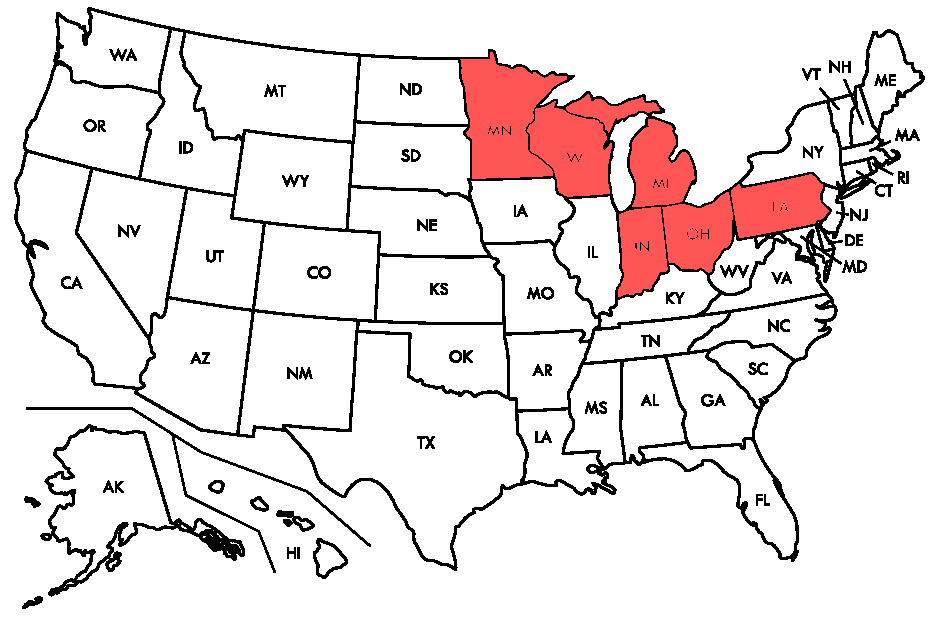
\includegraphics[width=0.65\linewidth, trim={0cm 0cm 0cm 0cm},clip]{gfx/Chapter5/Blank_US_map_borders_labelsClean.pdf} 
	\caption{States of the Great Lakes region studied in this work.}
	\label{fig:states}
\end{figure}

The CAFOs considered for the deployment of livestock waste treatment processes are those livestock facilities with more than 300 animal units \citep{CAFO_definition} reported in the National Pollutant Discharge Elimination System (NPDES) by the US EPA in the 
%Great Lakes area (i.e. Minnesota, Indiana, Ohio, Pennsylvania, Wisconsin, and Michigan)
states under evaluation. An animal unit is defined as an animal equivalent of 1,000 pounds live weight \citep{animal_unit_definition}. There are 2,217 CAFOs considered in total.
%The state
%%s
%of Illinois
%%and New York, as well as the Ontario province in Canada, are 
%is not part of this study due to the lack of reliable data about CAFOs.
The animal number, manure generated, and phosphorus releases by CAFOs in the studied states are reported in Table \ref{table:GreatLakes_manure}.

\begin{table}[h]
	\centering
	\caption{Livestock residues and phosphorus releases by CAFOs in the Great Lakes area.}
	\label{table:GreatLakes_manure}
	\resizebox{\columnwidth}{!}{
		\begin{tabular}{@{}ccccccc@{}}
			\toprule
			& Pennsylvania & Ohio     & Indiana  & Michigan & Minnesota & Wisconsin \\ \midrule
			Number of CAFOs & 131 & 53 & 119 & 144 & 1,487 & 283 \\
			\midrule
			Total animal units                                                                      & 196,617      & 128,008  & 187,355  & 354,460  & 943,094   & 744,015   \\ 
			Dairy animal units (\%)                                                                 & 85.06       & 79.17  & 81.93  & 87.90  & 45.43   & 98.38   \\
			Beef animal units (\%)                                                                  & 14.94       & 20.83   & 18.07   & 12.10   & 54.57   & 1.62    \\
			
			\midrule
			
			\begin{tabular}[c]{@{}c@{}}Manure generated\\ (kt/year)\end{tabular}                    & 2.60$\cdot 10^3$     & 1.68 $\cdot 10^3$ & 2.48$\cdot 10^3$ & 4.76$\cdot 10^3$ & 1.13$\cdot 10^{4}$  & 1.03$\cdot 10^{4}$  \\
			
			\midrule
			
			\begin{tabular}[c]{@{}c@{}}Phosphorus releases\\ (t/year)\end{tabular}                 & 2.08$\cdot 10^3$     & 1.34$\cdot 10^3$ & 1.98$\cdot 10^3$ & 3.80$\cdot 10^3$ & 9.02$\cdot 10^3$  & 8.20$\cdot 10^3$  \\ 		
			
			\midrule
			
			\begin{tabular}[c]{@{}c@{}}Reference\end{tabular}                 & 1     & 2 & 3 & 4 & 5  & 6  \\ 			
			\bottomrule
	\end{tabular}}
	\begin{tablenotes}
		\small
		\item \textsuperscript{1} \protect\citet{Pennsylvania_CAFOS}.
		\item \textsuperscript{2} \protect\citet{Ohio_CAFOS}.
		\item \textsuperscript{3} \protect\citet{Indiana_CAFOS}.
		\item \textsuperscript{4} \protect\citet{Michigan_CAFOS}.
		\item \textsuperscript{5} \protect\citet{Minnesota_CAFOS}.
		\item \textsuperscript{6} \protect\citet{Wisconsin_CAFOS}.
	\end{tablenotes}
\end{table}

\section{Results and discussion}
The results of the implementation and allocation of incentives for phosphorus recovery are shown in this section.
%The phosphorus recovered through the installation of P recovery systems in the Great Lakes area, as well as the capital and operating costs associated with these processes if no incentives are considered, are reported in \citet{Tool}.
The results regarding the techno-economic assessment of the different processes, technology selection, and phosphorus recovered can be found in \citet{Tool}.

\subsection{Single incentives}
%In this section, the effect of the implementation of single P credits or REC incentives is studied. The capital and operating costs associated with the installation of P recovery systems if no incentives are considered are reported \citet{Tool}.
\subsubsection{Effect of P credits}
The effect of applying P credits on the economic performance of nutrient management systems has been studied. Revenues from struvite sales are also considered in those CAFOs installing struvite production technologies. Since in this first scenario only the effect of P credits is studied, incomes from electricity production are excluded; and therefore, the nutrient management systems are not integrated with biogas production. The effect of the value of P credits over the profitability of the nutrient recovery systems is shown in Fig \ref{fig:NoREC}, where the distribution of CAFOs size is shown using boxplots. It can be observed that, for P credits values strictly below 11 USD per kg of recovered phosphorus, the proportion of profitable P recovery processes (those installed processes whose incomes are larger than their operating expenses) is small and constant. However, when the value of the incentive is set at 11 USD per kg of recovered phosphorus, the increase in the number of profitable processes is very significant for all states except Minnesota, which CAFOs median size is the smallest. For states with large CAFOs, i.e. Michigan, Ohio and Wisconsin, the percentage of profitable processes can reach around 80\% under high P credits; while for Indiana and Pennsylvania, with medium-size CAFOs, around 40\% are profitable. For P credits of 22 USD per kg of recovered phosphorus, there is an additional 25\% increase of profitable nutrient recovery systems in those states with large CAFOs. In the states with medium size CAFOs the increase of profitable processes is also very significant, reaching approximately 80\% of the studied CAFOs. Finally, for the case of Minnesota, there is a large increase in the profitable P recovery systems installed as well, reaching near the 60\% of the CAFOs studied.

\begin{figure}[h!]
	\centering
	\begin{subfigure}[t]{0.85\textwidth}
		\centering
		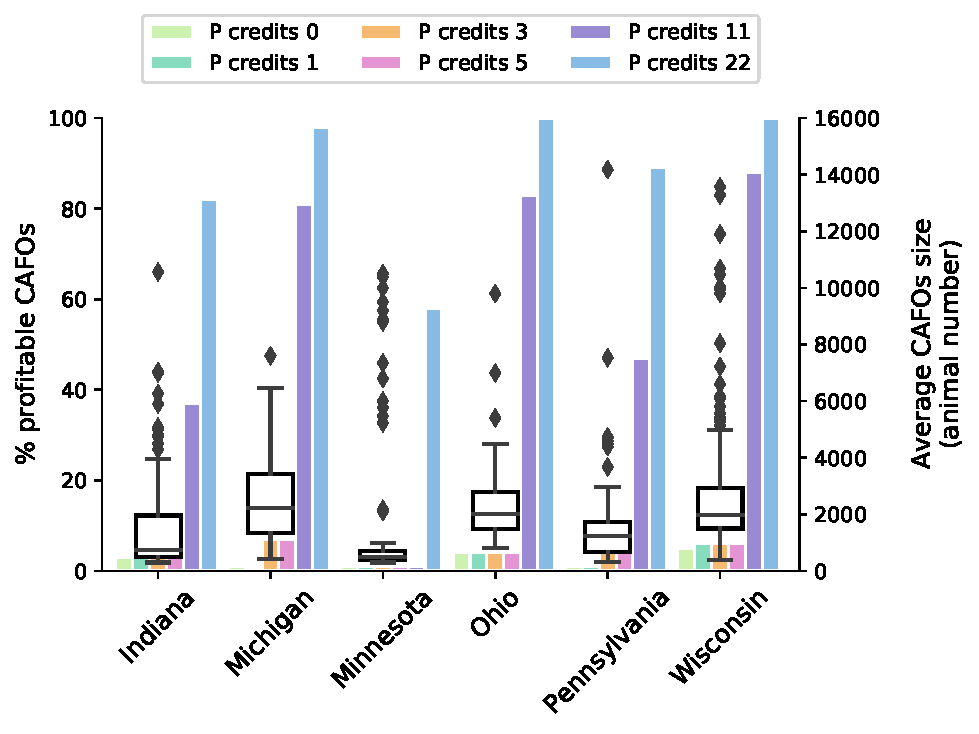
\includegraphics[width=\linewidth]{gfx/Chapter5/REC0DataAnalysis__PercProfitableStatesClean.pdf} 
		\caption{P credits $\left(\frac{\text{USD}}{\text{kg}_\text{P recovered}}\right)$}
		\label{fig:NoREC}
	\end{subfigure}
	\begin{subfigure}[t]{0.85\textwidth}
		\centering
		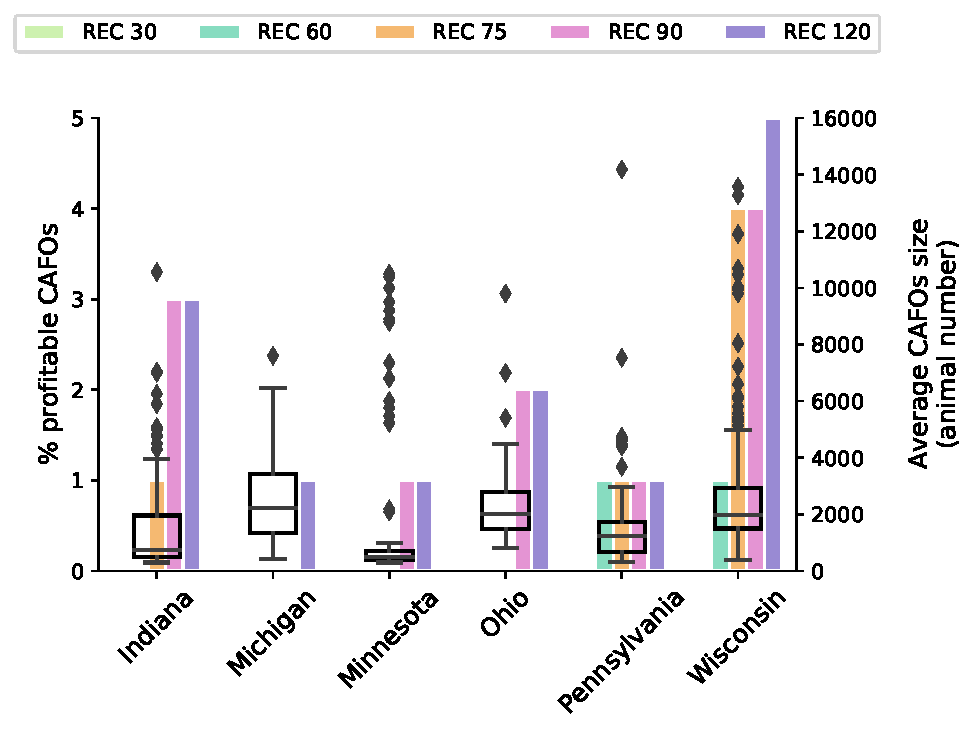
\includegraphics[width=\linewidth]{gfx/Chapter5/PC0DataAnalysis__PercProfitableStatesClean.pdf}
		\caption{REC $\left(\frac{\text{USD}}{\text{MWh}}\right)$}
		\label{fig:NoPCredits}
	\end{subfigure}
	
	\caption{Distribution of profitable phosphorus recovery processes in the Great Lakes area for the scenarios considering phosphorus credits and renewable energy credits. The box-plots represent the distribution of CAFOs size in each state.}
	\label{fig:SingleIncentives}
\end{figure}

\subsubsection{Effect of renewable energy certificates}\label{section:Electricity_price}
The effect of REC in the implementation of P recovery systems is studied in this section. Integration of biogas production with P recovery processes is considered in all the cases studied in this scenario. In addition to revenues obtained from RECs, incomes from the sales of struvite produced by the phosphorus recovery processes have been considered as well. The effect of P credits is excluded in this scenario.

Figure \ref{fig:NoPCredits} shows the percentage of profitable P recovery processes for each studied state together with the distribution of the size of CAFOs. As it can be observed, the impact of the incomes from electricity in the economic performance is much less significant than the effect of P credits given the incentive ranges considered. Only the largest CAFOs, most of which represent outliers in the distribution of CAFOs size, are profitable when prices equal to or above 75 USD/MWh are considered. The large CAPEX prevent the economic feasibility of biogas production in small and medium CAFOs. Therefore, only large-scale CAFOs can benefit from the operation of biogas processes to cover the cost of P recovery systems via biogas-based electricity production.

\subsection{Combined effect of incentives for phosphorus and renewable electricity recovery}\label{section:CombIncent}
Synergies derived from the combination of P credits and RECs might be obtained when integrating phosphorus recovery technologies with biogas production and upgrading processes.
However, since the deployment of the biogas processes involves large investments and considerable operating costs, a detailed analysis must be conducted to identify the most cost-effective incentives policy. 

The results obtained from combining the incentive schemes described in previous sections are shown in Figure \ref{fig:AllScenarios}. The fraction of profitable processes is shown in Figure \ref{fig:PercProfitableStates_AllScenarios}, which are defined as those CAFOs with positive net incomes. It can be observed that, if the value of P credits and RECs are set similar to the market prices (i.e. 1 USD/$\text{kg}_\text{P recovered}$ and 60-75 USD/MWh respectively), the fraction of profitable processes is very low. Wisconsin is the state with the largest share of profitable P recovery processes under this scenario, which is 4-5\% of the total CAFOs.

Phosphorus credits have a larger impact on the profitability of nutrient management systems, near to 100\% for P credits of 22 USD/${\text{kg}_\text{P recovered}}$ for states with large CAFOs (i.e. Michigan, Ohio and Wisconsin). The price of electricity has a weak influence on the profitability of the deployed systems in these scenarios. For states with medium-size CAFOs, Indiana and Pennsylvania, the share of profitable processes is around 80-85\%. For Minnesota, which is the state with the smallest median CAFOs size, the share is 58\%. Therefore, the installation of AD processes has a significant negative impact in the states with small and medium size CAFOs due to the lack of economies of scale. A similar behavior is found when the value of phosphorus credits is reduced to 11 USD/${\text{kg}_\text{P recovered}}$.

\begin{figure}[h!]
	\centering
	\begin{subfigure}[t]{\textwidth}
		\centering
		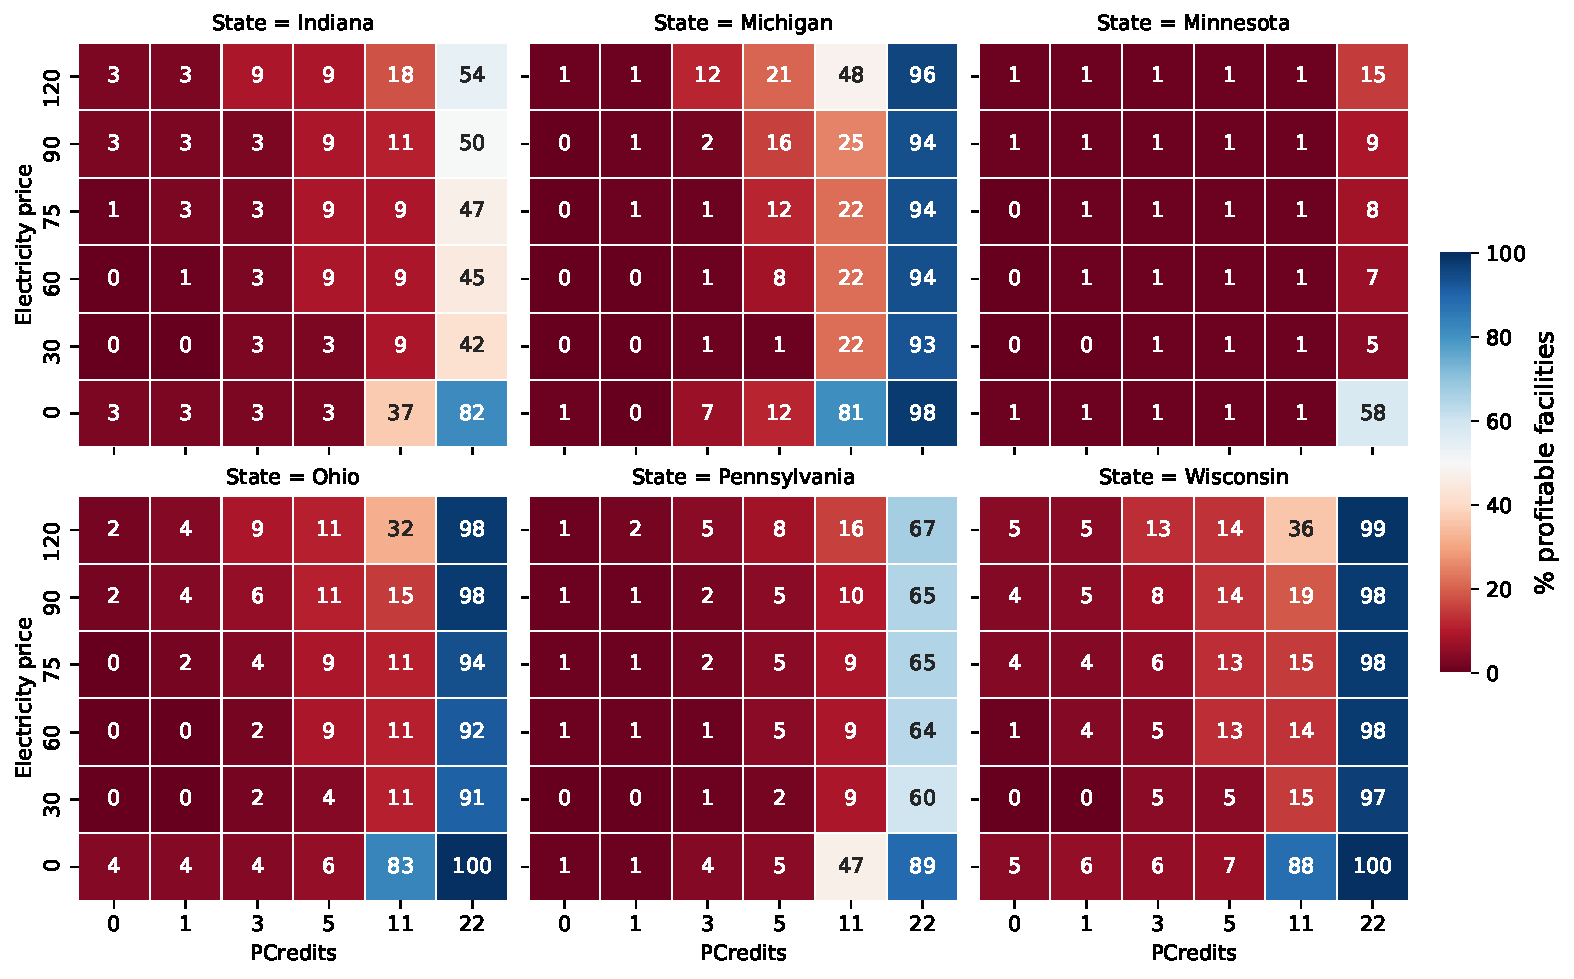
\includegraphics[width=\linewidth]{gfx/Chapter5/DataAnalysisProfitableClean.pdf} 
		\caption{Percentage of profitable phosphorus recovery processes}
		\label{fig:PercProfitableStates_AllScenarios}
	\end{subfigure}
	\par\bigskip
	\begin{subfigure}[t]{\textwidth}
		\centering
		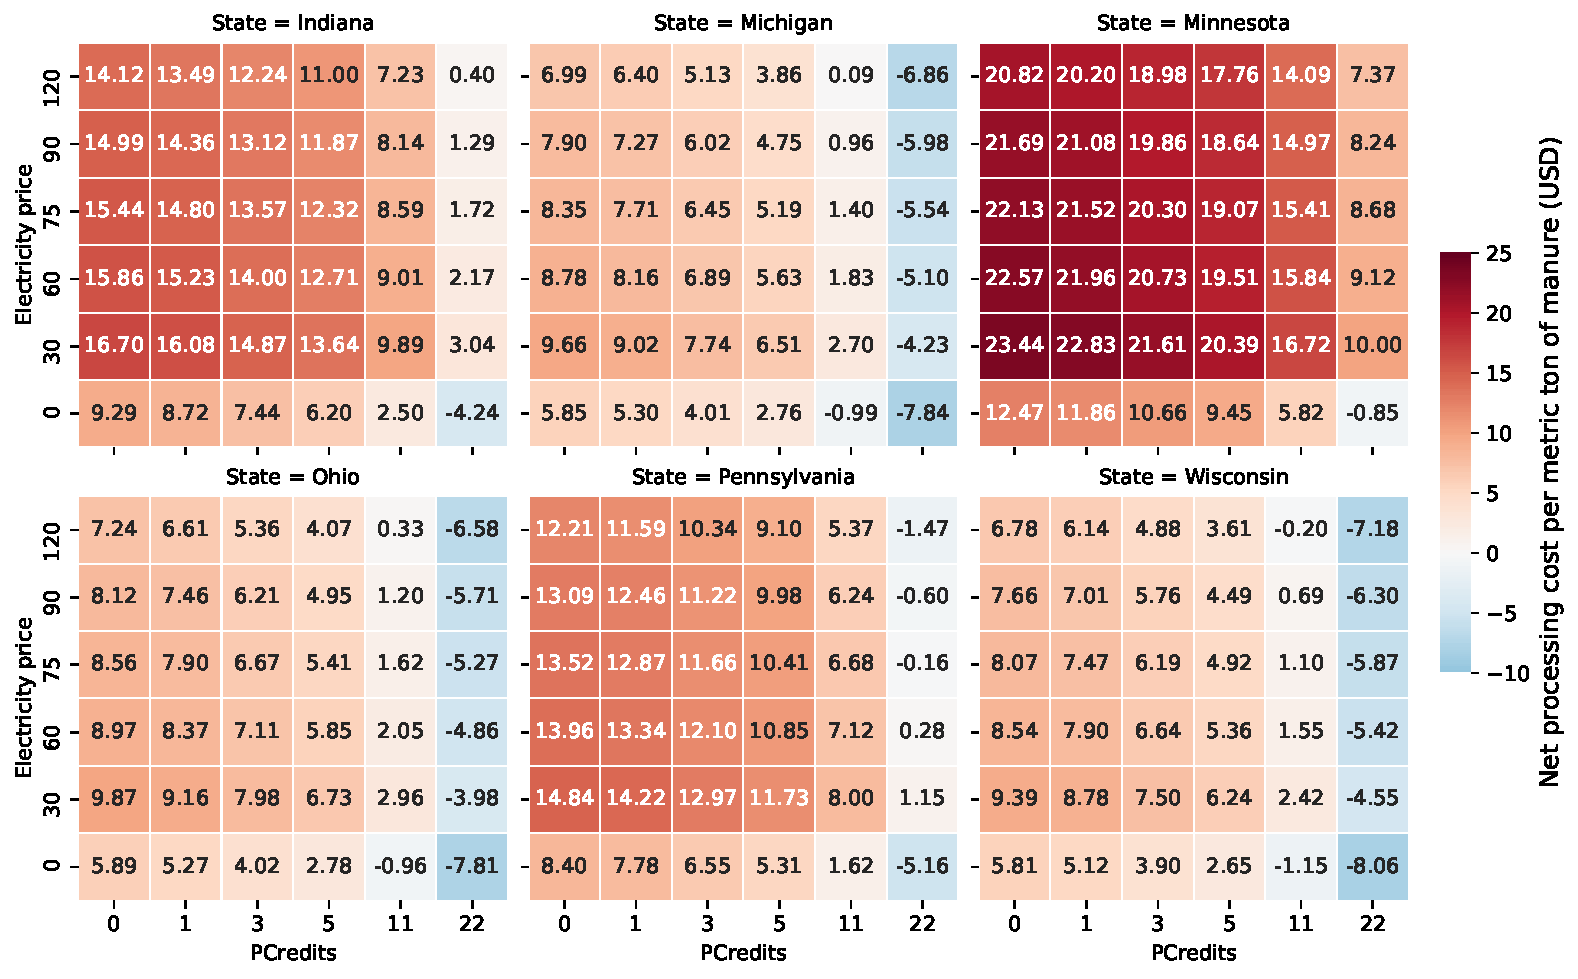
\includegraphics[width=\linewidth]{gfx/Chapter5/TAC_tonManureClean.pdf}
		\caption{Net processing cost per metric ton of manure (USD)}
		\label{fig:TAC_kgManure_AllScenarios}
	\end{subfigure}
	
	\caption{Economic evaluation of P recovery processes for the different incentives scenarios studied}
	\label{fig:AllScenarios}
\end{figure}

This pattern is reverted when P credits of 3-5 USD/${\text{kg}_\text{P recovered}}$ are considered. For these scenarios the share of profitable processes is considerably reduced compared to the previous scenarios. Actually, for Indiana, Minnesota, and Ohio, there is no difference between setting phosphorus credits incentives below 5 USD/${\text{kg}_\text{P recovered}}$ and the case considering no P credits (where the only income of phosphorus recovery is from the sales of nutrient-rich products obtained). However, in all states except Minnesota, the amount of profitable systems increases for electricity prices larger than 60 USD/MWh, reaching a share of P recovery processes with positive net incomes up to 22 \% for Michigan. For the scenario considering P credits of 1 USD/${\text{kg}_\text{P recovered}}$, only Ohio shows a slight improvement in the fraction of profitable facilities if the production of electricity is also considered. Therefore, there is a threshold for P credits between 1 and 3 USD/$\text{kg}_\text{P recovered}$ below which no improvement in the fraction of profitable P recovery systems is observed. For those scenarios where no incentive for phosphorus recovery is considered, the results obtained have been previously described in Section \ref{section:Electricity_price}. It is interesting to note that, as a consequence of the large capital and operating expenses of AD processes, the economic performance of the scenarios considering only P recovery systems is at least as profitable as the profitability of the scenarios considering biogas generation associates the largest REC incentives.

The net treatment cost per ton of manure processed captures the perspective of CAFOs owners on P recovery. It is defined as the difference between the revenues (sum of struvite sales, $R_{c}$ (USD/year), and incentives, $I_{c}$ (USD/year)) and the operating expenditures of livestock treatment processes, $OPEX_{c}$ (USD/year), as shown in Eq. \ref{eq:NetTreatCost}. $F_{\text{manure}_{c}}$ denotes the mass flow of manure processed in ton/year.

\begin{align}
& \text{Net treatment cost}_c \left(\frac{\text{USD}}{\text{t}_{\text{manure}}}\right) = \frac{R_{c} + I_{c} - OPEX_{c}}{F_{\text{manure}_{c}}} \label{eq:NetTreatCost}
\end{align}

%\begin{figure}[H]
%	\centering
%	\begin{subfigure}[t]{0.89\textwidth}
%		\centering
%		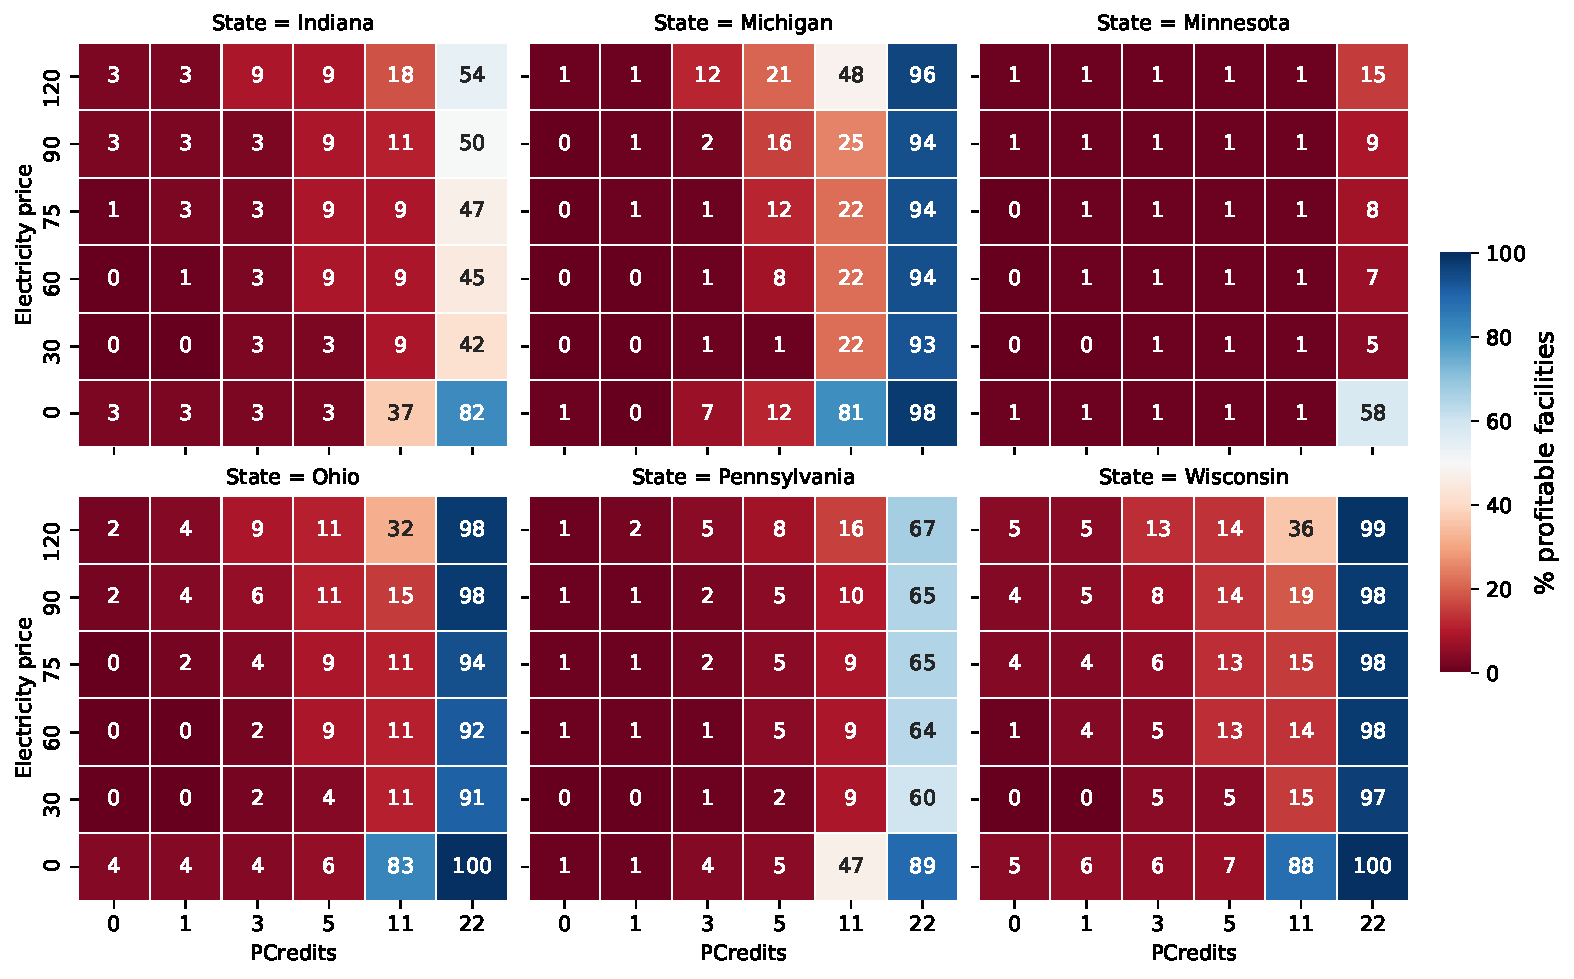
\includegraphics[width=\linewidth]{DataAnalysisProfitable.pdf} 
%		\caption{Percentage of profitable phosphorus recovery processes}
%		\label{fig:PercProfitableStates_AllScenarios}
%	\end{subfigure}
%	\par\bigskip
%	\begin{subfigure}[t]{0.89\textwidth}
%		\centering
%		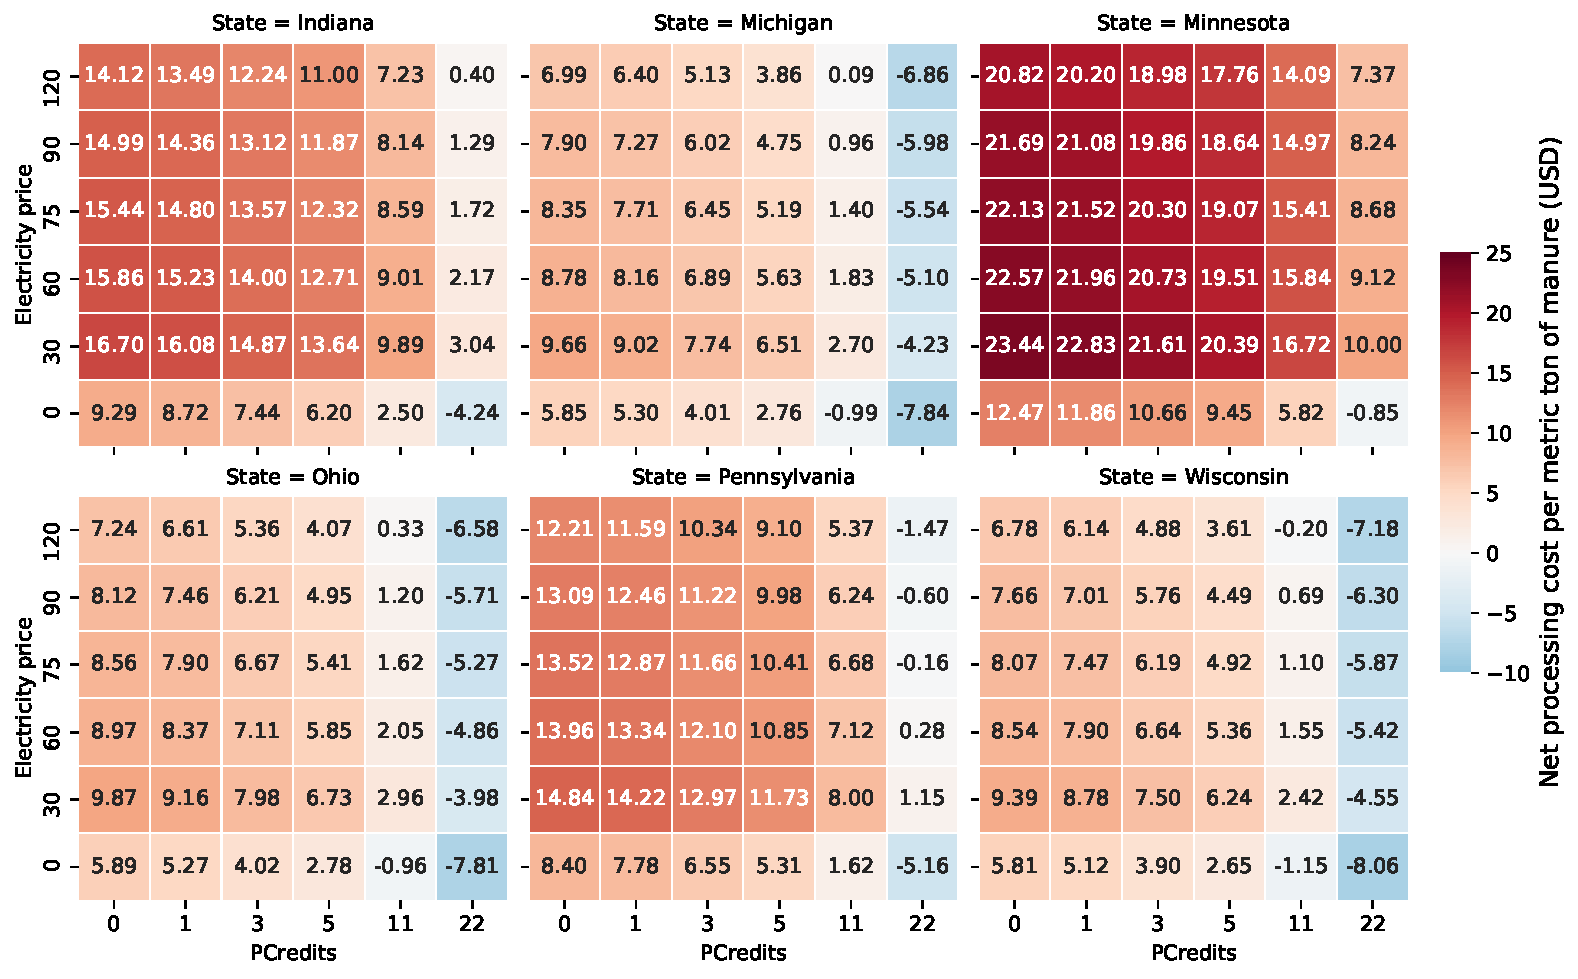
\includegraphics[width=\linewidth]{TAC_tonManure.pdf}
%		\caption{Net processing cost per metric ton of manure (USD)}
%		\label{fig:TAC_kgManure_AllScenarios}
%	\end{subfigure}
%	
%	\caption{Economic evaluation of P recovery processes for the different incentives scenarios studied}
%	\label{fig:AllScenarios}
%\end{figure}

The results obtained in terms of net treatment cost are illustrated in Figure \ref{fig:TAC_kgManure_AllScenarios}. They  show a base cost for the recovery of phosphorus between 5.81 and 12.47 USD per ton of processed manure if no incentives or anaerobic digestion stages are considered. From this base case, it can be observed that the costs vary following the same pattern as the fraction of profitable processes described previously. The installation of biogas processes is not profitable by itself, increasing the processing costs by 1.2-1.9 times over the base case if no P credits are considered, and it is only beneficial for specific scenarios which have large size CAFOs, and moderate P credits ($>$3 USD/${\text{kg}_\text{P recovered}}$) and electricity incentives ($>$60 USD/MWh). The scenarios combining states with large CAFOs and high value for P credits, and the optional production of renewable energy from biogas result in negative processing costs. This means that phosphorus recovery results in profits for the CAFO. We note that, as the analysis of the different scenarios is carried out at the state level, a negative processing cost indicate that, under certain schemes for incentives, the profitable P recovery processes are able to balance out the non-profitable ones in the state.

It is worth noting that the results reveal that in the largest CAFOs the recovery of phosphorus is more economically feasible, due to the economies of scale. At the same time, however, these large-scale CAFOs also represent the major current environmental threats due to the release of larger amounts of phosphorus. The reduction of phosphorus recovery cost and the abatement of nutrient releases might be interpreted as an opportunity for CAFOs to increase their capacity. However, further issues related to resource requirements and additional environmental impacts must be considered before stating that the current capacity of CAFOs can be increased, including water availability, greenhouse gas emissions, and odor releases.
%In addition, animal health issues could arise as a consequence of the increase of the animals in a confined facility.

\subsection{Environmental cost-benefit analysis}
CAFOs are an environmental concern in terms of nutrient pollution as a consequence of the high spatial concentration of animals, resulting in large releases of phosphorus. 
The long-term environmental impact of phosphorus releases result in large economic losses, accounting for the remediation cost of environmental degradation and the economic impact on the local population affected by HABs. Therefore, an analysis for the cost-effectiveness of the total cost involved in phosphorus recovery, including the amortization of the investment, operating costs, and total cost of incentives, can show the economic advantages of phosphorus recovery. 

\begin{align}
& \text{Total treatment cost}_{c} \left(\frac{\text{USD}}{\text{kg}_{\text{P recovered}}}\right) = -R_{c} + I_{c} + OPEX_{c} \label{eq:TotTreatCost}
\end{align}

\begin{figure}[h!]
	\centering
	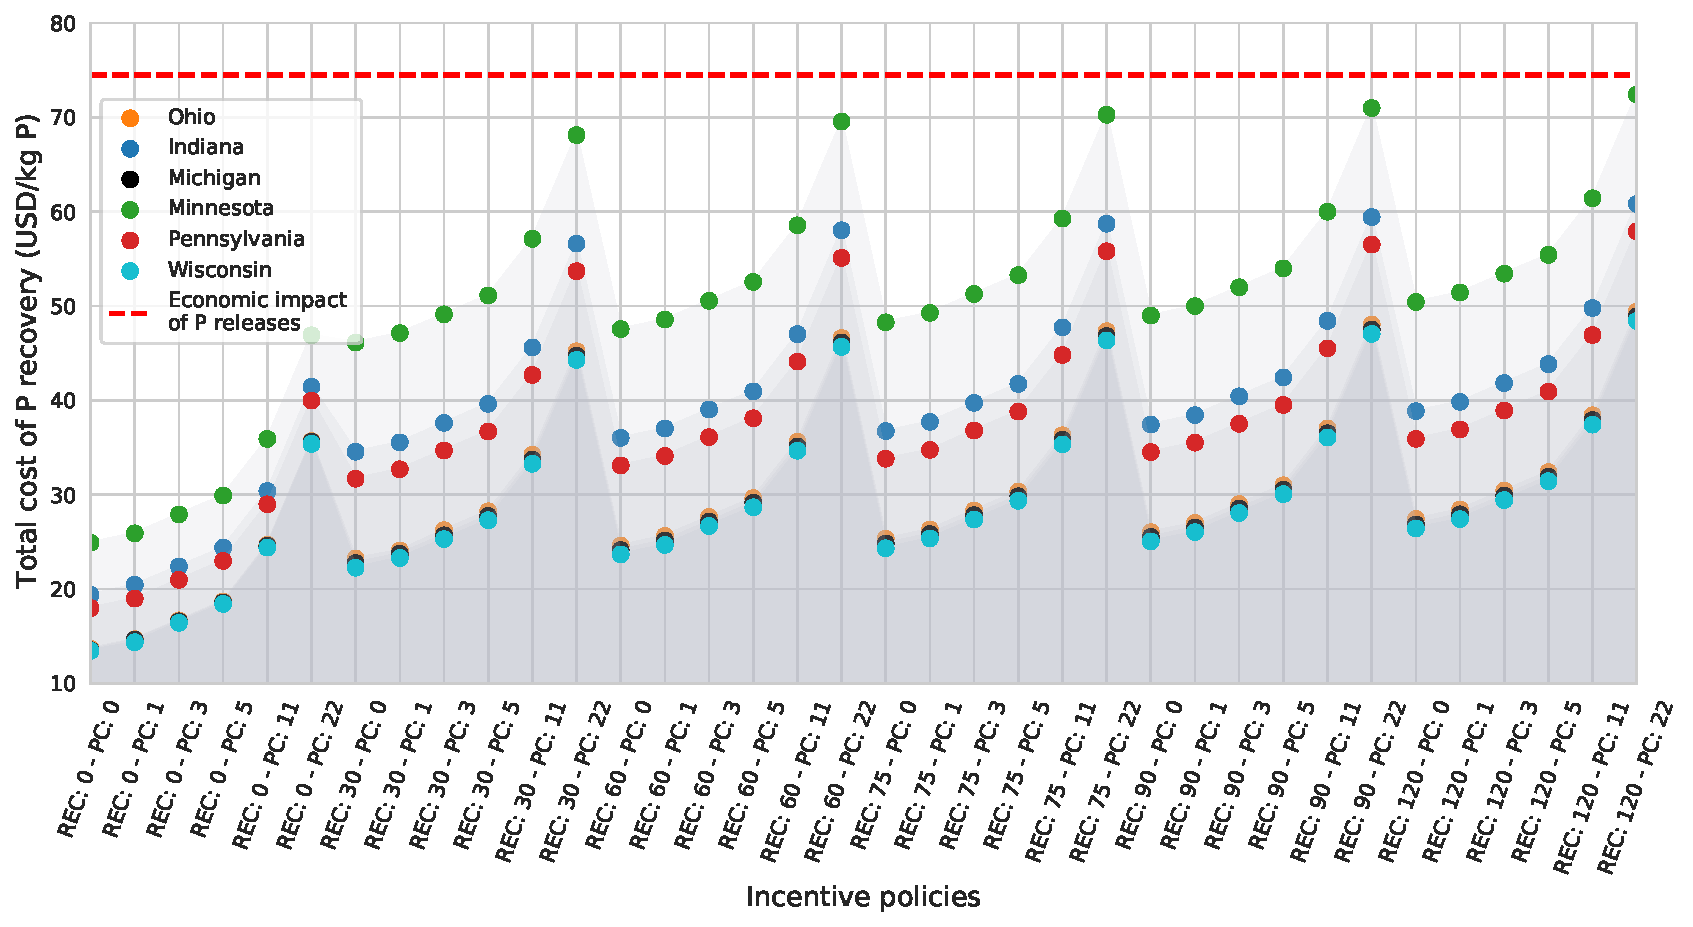
\includegraphics[width=\linewidth]{gfx/Chapter5/TotalCost_kgPRecoveredAllStatesv2Clean.pdf} 
	
	\caption{Comparison of the total cost of phosphorus recovery for each scenario assessed and the environmental remediation cost due to phosphorus releases. \textit{REC} denotes the electricity incentive values considered in USD/MWh, and \textit{PC} denotes the value of phosphorus credits in USD/${\text{kg}_\text{P recovered}}$. The red dotted line represents the economic losses due to phosphorus releases to the environment.}
	\label{fig:plot_scenarios}
\end{figure}

Figure \ref{fig:plot_scenarios} shows the total cost of phosphorus recovery under different policies, defined in Eq. \ref{eq:TotTreatCost}, compared with the economic losses due to phosphorus releases into the environment. It can be observed that all scenarios studied result in a phosphorus recovery cost lower than the economic losses due to phosphorus releases, estimated in 74.5 USD per kg of phosphorus released by \citet{Sampat2020}. Phosphorus recovery is, therefore, more cost-effective than its release to the environment. The lowest total cost for phosphorus recovery is obtained in the scenario not involving any incentive (\textit{REC: 0 - PC: 0}), resulting in costs between 3 and 5 times lower than the economic cost of phosphorus release to the environment. The application of incentives increases the total monetary cost of phosphorus recovery.
%, mainly driven by the application of phosphorus credits.
However, since incentives are an income for the owners of livestock facilities, the economic cost of nutrient management systems for the owners of CAFOs is progressively reduced, increasing the number of profitable P recovery systems, and reducing the recovery cost of phosphorus, as it is shown in Fig. \ref{fig:AllScenarios}.

The role of the size of CAFOs in the cost of phosphorus recovery can be also observed in this study. In accordance, with the results shown in previous sections, those states with larger average size of CAFOs, such as Wisconsin, Ohio, and Michigan, have recovery costs significantly lower than the states where medium and small size CAFOs are predominant. 
%It is worth noting that the total cost of phosphorus recovery is lower than the economic losses due to the release of phosphorus to the environment for all the evaluated states and policies.



\subsection{Fair distribution of incentives}
The effect of different incentive schemes has been previously discussed, revealing that the P recovery systems in small CAFOs require significant economic support in the form of incentives to balance the monetary losses, while in the largest CAFOs these systems can be self-profitable. This situation leads to the problem of the fair distribution of available incentives, which is particularly relevant in the case that the available budget is not sufficient to cover the operating expenses of the unprofitable P recovery processes. In this section, the minimum necessary incentives for all P recovery systems in the studied area to reach the economical neutrality (i.e., no economic profits or losses are obtained) is firstly determined. In a second stage, a fairness-guided distribution of incentives among CAFOs is studied when the available incentives are lower than the monetary amount determined, i.e., they are not sufficient to cover the operating expenses of unprofitable processes. Due to the marginal benefits obtained by installing AD processes, as described in Section \ref{section:CombIncent}, the implementation of only P recovery systems is assumed in both studies, and therefore only incentives for P recovery are considered.

The minimum cost of incentives necessary
%for covering 
to cover for the economic losses of unprofitable processes, estimated in 222.6 million USD, is determined through the formulation of an optimization problem. The objective function of this problem minimizes the incentives used, Eq. \ref{eq:objMinIn}, subject to achieve the economical neutrality, Eq. \ref{eq:cons1MinIn}. Here, $\mathcal{C}$ denotes the set of CAFOs studied, $I_{c}$ the  incentives allocated, and $OPEX_{c}$ and $R_{c}$ the operating expenses and revenues of the P recovery system installed in each CAFO $c$ respectively.

\begin{subequations}
	\begin{align}
	& \text{min} \ \ \sum_{c \in \mathcal{C}} I_{c}  \label{eq:objMinIn} \\
	& \text{s.t.} \ \ I_{c} + R_{c} - OPEX_{c} \geq 0 \label{eq:cons1MinIn}
	\end{align}
\end{subequations}

The results obtained, shown in Figure \ref{fig:MinIncent}, reveal the crucial role of the economies of scale in the amount of incentives that must be deployed to cover the economic losses of P recovery systems. We note that the discrepancies of incentives for CAFOs of similar size that can be observed in the figure are due to the different technology installed. The selection of different P recovery processes for CAFOs of similar size is based on the eutrophication risk of each watershed, 
as described in \citet{Tool}.
%see Section 2.4 of the Supplementary Material. 
It can also be observed that 99.9\% of CAFOs require incentives below the P releasing cost to the environment. A correlation to estimate the amount of incentives needed to cover the operating expenses as a function of CAFOs capacities is proposed in Eq. \ref{eq:CorrMinIn} , where $AU_{c}$ denotes the animal units of CAFO $c$.

\begin{figure}[h!]
	\centering
	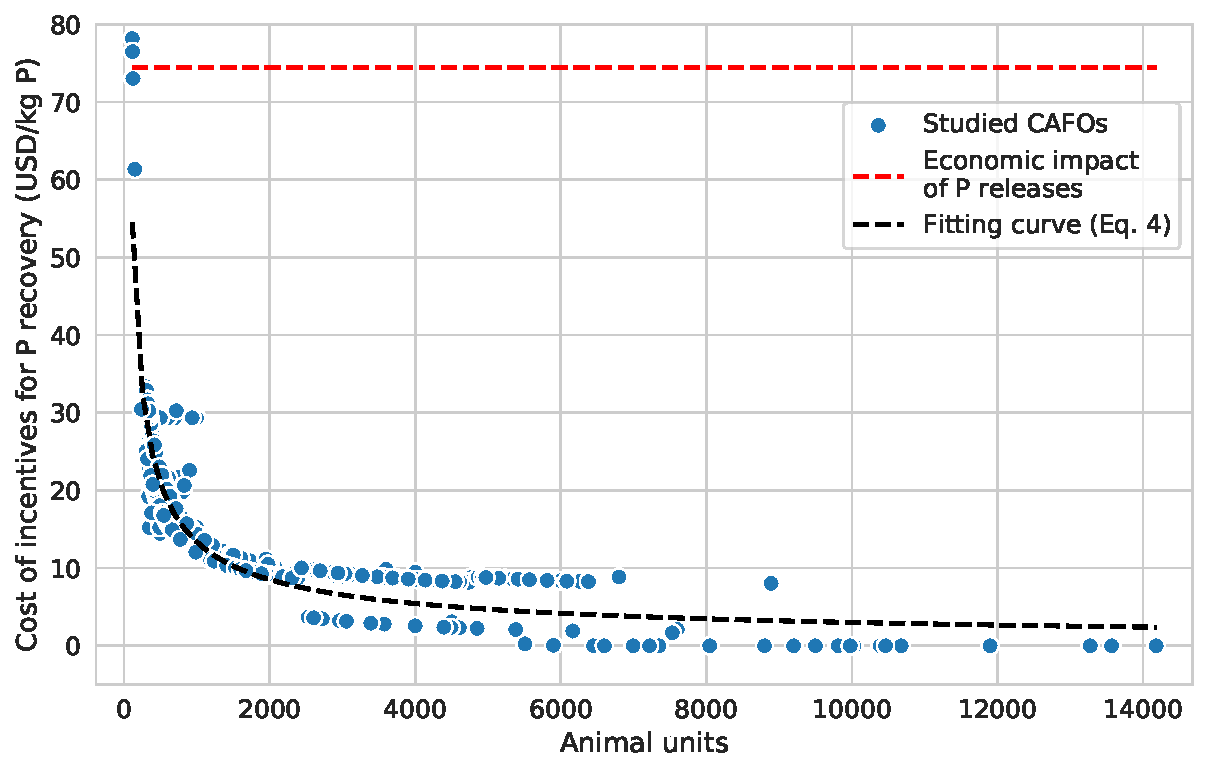
\includegraphics[width=0.9\linewidth, trim=0cm 0cm 0cm 0cm, clip]{gfx/Chapter5/MinIncentClean.pdf}
	\caption{Allocation of incentives for achieving the economic neutrality of nutrient recovery systems minimizing the total cost of incentives.}
	\label{fig:MinIncent}
\end{figure}

\begin{align}
& I_{c} \ \left(\frac{\text{USD}}{\text{kg P}}\right) = \frac{3.383 \cdot 10^6}{1+\left(AU_{c} \cdot 2.223\cdot 10^5 \right)^{0.647}} \label{eq:CorrMinIn} 
\end{align}

The fair allocation of incentives when the monetary amount available is not sufficient to cover the expenses of all P recovery processes has been addressed by using the Nash allocation scheme. The Nash approach has been selected because this scheme is able to capture the scales of the different stakeholders (CAFO facilities) in order to achieve a fair distribution of a certain resource (incentives), as it was demonstrated by \citet{sampat2019fairness}. This scheme is formulated in Eqs. \ref{eq:objNashIn}-\ref{eq:cons1NashIn}, where $I_{\text{available}}$ denotes the available incentives.

\begin{align}
& \text{Net revenue before incentives}_{c} \left(\frac{\text{USD}}{\text{year}}\right) = R_{c} - OPEX_{c} \label{eq:NetRevBeforeInc}
\end{align}

Figure \ref{fig:NashIncent} illustrates the distribution of incentives as a function of the net revenues of the P recovery system installed in each CAFO $c$ before any incentive is applied, Eq. \ref{eq:NetRevBeforeInc}.

\begin{subequations}
	\begin{align}
	& \text{max} \ \ \sum_{c \in \mathcal{C}} \text{ln} \left(I_{c} + R_{c} - OPEX_{c}\right)  \label{eq:objNashIn} \\
	& \text{s.t.} \ \ \sum_{c \in \mathcal{C}} I_{c} \leq I_{\text{available}} \label{eq:cons1NashIn}
	\end{align}
\end{subequations}

\begin{figure}[h!]
	\centering
	\begin{subfigure}[t]{0.89\textwidth}
		\centering
		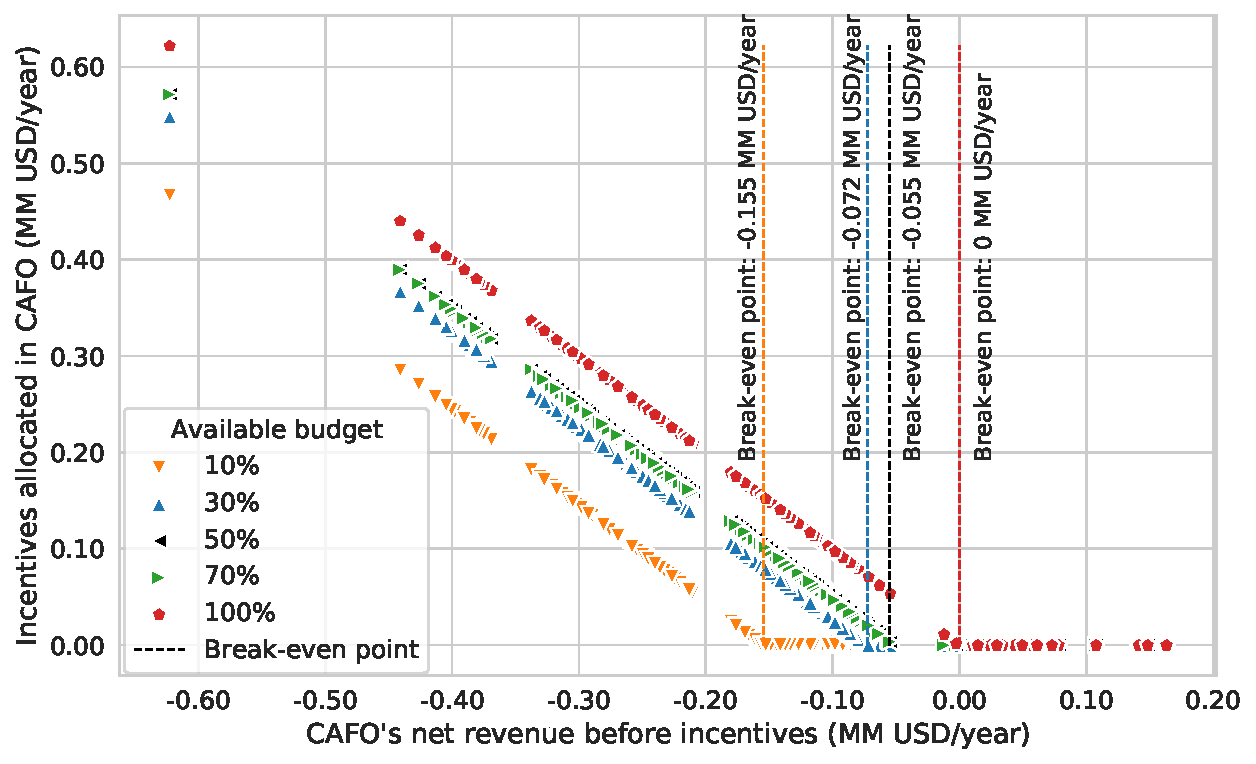
\includegraphics[width=\linewidth]{gfx/Chapter5/NashIncentClean.pdf} 
		\caption{Distribution of incentives}
		\label{fig:NashIncent}
	\end{subfigure}
	\par\bigskip
	\begin{subfigure}[t]{0.89\textwidth}
		\centering
		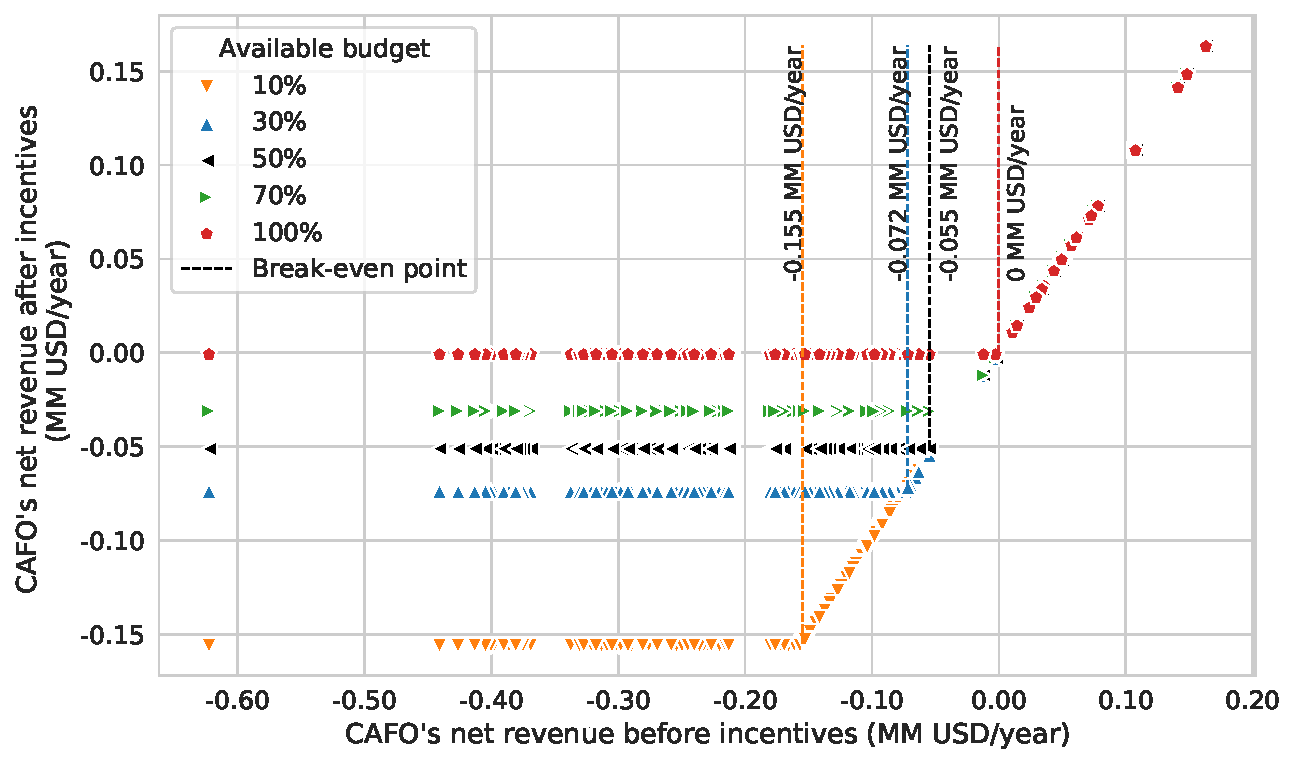
\includegraphics[width=\linewidth]{gfx/Chapter5/NashIncentv2Clean.pdf}
		\caption{CAFOs net revenue after incentives allocation}
		\label{fig:NashRevenues}
	\end{subfigure}
	
	\caption{Distribution of incentives considering the Nash allocation scheme. Scenarios assuming available incentives equal to the 10\%, 30\%, 50\%, 70\%, and 100\% of the incentives needed to cover the economic losses of unprofitable P recovery systems in the Great Lakes area are illustrated.}
	\label{fig:AllNash}
\end{figure}

The cases where the available budget are the 10\%, 30\%, 50\%, 70\%, and 100\% of the incentives needed to cover the economic losses of unprofitable CAFOs are analyzed (22.3, 66.8, 111.3, 155.8 and 222.6 MM USD respectively). The last case is equivalent to the scenario studied above. It can be observed that the available incentives are allocated accordingly to the net revenues of each CAFO, promoting the allocation of larger incentives to the less profitable P recovery processes. Since the available incentives are limited, a break-even point determining the profitability level of the P recovery systems below which the incentives should be allocated is set for each scenario. As a result, the fewer incentives available, the more restrictive the break-even point is. Additionally, it can be observed that the displacement of the break-even points is progressively reduced as the available incentives increase, resulting in a marginal improvement between the scenarios considering the 50\% and 70\% of the economic resources needed to guarantee the economic neutrality of the nutrient management systems. In Figure \ref{fig:NashRevenues} we observe that, for each case evaluated, the allocation of limited incentives under the Nash scheme results in a uniform net revenue for those CAFOs receiving incentives. Additionally, we note that the economic losses have been mitigated in these facilities by the allocation of incentives. However, they are unable to be profitable due to the limited budget available. In addition, a correlation to estimate the fairness point as a function of available incentives has been developed based on these results, Eq. \ref{eq:FairnessPoint}.

\begin{align}
& \text{Break-even point}_c \ \left(\frac{\text{USD}}{\text{year}}\right) = -2.482\cdot10^{5} \cdot \left(0.955^{\left(I_{\text{available}}\left( \% \right) \right)}\right) \label{eq:FairnessPoint}
\end{align}

\section{Conclusions}
%The application of different incentives to promote the implementation of nutrient management systems at CAFOs is studied in this work, including the potential integration of phosphorus recovery technologies with the production of renewable electricity from biogas. 
Nowadays, nutrient releases from CAFOs into the environment in the form of manure application in croplands are restricted by regulations in the US and the UE. Moreover, the US National Pollutant Discharge Elimination System requires the CAFOs to include the necessary provisions for avoiding the harmful effects of the discharges on water and human health, but no specific methods or processes, including nutrient management systems, are defined under current regulation. This work aims at analyzing incentive policies for the implementation of phosphorus recovery systems for the abatement of nutrient releases from CAFOs, including the potential integration of phosphorus recovery technologies with the production of renewable electricity from biogas.

The results reveal that the recovery of phosphorus is more economically feasible in the largest CAFOs due to the economies of scale. The deployment of phosphorus recovery processes is self-profitable through struvite sales only for the largest P recovery processes, which represent less than the 5 \% over the total CAFOs in all the studied states. However, the application of P credits increases the fraction of profitable processes around to 100\% in the states with large-size CAFOs (Michigan, Ohio and Wisconsin), and up to 80\% for the states with medium-size CAFOs (Indiana and Pennsylvania).
The incentives necessary for covering the economic losses of unprofitable CAFOs estimated in 222.6 million USD.
The integration of phosphorus recovery technologies with anaerobic digestion and biogas upgrading processes does not result in any practical improvement in terms of economic performance unless incentives for phosphorus recovery are considered, since the revenues from electricity sales can not cover the investment and operating cost of these processes given current market values.

The total cost of phosphorus recovery, including the investment amortization, operating costs, and total cost of incentives is lower than the long-term economic losses due to phosphorus pollution for all the evaluated states and policies, proving that sustainable nutrient management systems are economically and environmentally beneficial. Correlations to estimate the incentives necessary for P recovery systems to achieve economic neutrality has been also proposed. Additionally, the fair distribution of limited incentives has been studied, determining the break-even point for the allocation of monetary resources based on the availability of incentives. This information can be used to raise the debate on which stakeholders and by how much should cover the cost of phosphorus recovery from the livestock industry, and from a broader perspective, the cost of environmental remediation derived from the different environmental impacts caused by this sector. If no incentives are applied, small CAFOs are more negatively impacted by the cost of phosphorus recovery than larger CAFOs due to the economies of scale, resulting in comparative disadvantages between different livestock facilities. Therefore, implementing fair-distributed incentives to mitigate the economic impact of phosphorus recovery at CAFOs is needed. In the case that the budget needed for these incentives is provided by national or regional administrations, taxpayers are the ultimate funders of these incentives whether they
%are consumers of livestock products
receive benefits from the livestock industry. Conversely, specific taxes to livestock products can be proposed for funding phosphorus recovery, but they can lead to the rise of the livestock product prices, discouraging consumers demand, business profitability, and outsourcing. As a result, this scheme can result in a negative impact of phosphorus recovery in the economy of CAFOs through the decrease of products demand. Therefore, further economic studies are needed the determine the optimal funding scheme for phosphorus recovery incentives. In addition,
future work is aimed at assessing the effect of biomethane production in the economy of the waste treatment systems, and the integration within a logistics network model for the developing of nutrient pollution and ecosystem integrated responses at regional spatial resolution.

\section*{Acknowledgments} \label{section:AcknowledgmentsIncentives}
\addcontentsline{toc}{section}{Acknowledgments}
This research was supported in part by an appointment for E.M.H. to the Research Participation Program for the Office of Research and Development, US EPA, administered by the Oak Ridge Institute for Science and Education through Interagency Agreement No. DW-89-92433001 between the US Department of Energy and the US Environmental Protection Agency. E.M.H. and M.M. acknowledge funding from Junta de Castilla y Le\'{o}n, Spain, under grant SA026G18 and grant EDU/556/2019. Y.H. and V.M.Z. acknowledge funding from the U.S. Department of Agriculture, National Institute of Food and Agriculture, under grant number 2017-67003-26055.

\textbf{Disclaimer:} The views expressed in this article are those of the authors and do not necessarily reflect the views or policies of the U.S. EPA. Mention of trade names, products, or services does not convey, and should not be interpreted as conveying, official U.S. EPA approval, endorsement, or recommendation.

\section*{Bibliography}
\addcontentsline{toc}{section}{Bibliography}

\printbibliography[heading=none]
\end{refsection}